\documentclass[12pt,a4paper]{article}

% ==================== PACOTES ====================
\usepackage[utf8]{inputenc}
\usepackage[T1]{fontenc}
\usepackage[brazil]{babel}
\usepackage{graphicx}
\usepackage{amsmath,amssymb}
\usepackage{geometry}
\usepackage{fancyhdr}
\usepackage{hyperref}
\usepackage{caption}
\usepackage{subcaption}
\usepackage{indentfirst}
\usepackage{float}
\usepackage{siunitx}
\usepackage{booktabs}
\usepackage{array}
\usepackage{tabularx}
\usepackage{xcolor}

% ==================== CONFIGURAÇÕES DE PÁGINA ====================
\geometry{a4paper, top=3cm, bottom=2.5cm, left=3cm, right=2cm}

\pagestyle{fancy}
\fancyhf{}
\renewcommand{\headrulewidth}{0.6pt}
\fancyhead[L]{\includegraphics[height=1.1cm]{logo_utfpr.png}}
\fancyhead[c]{Eng. Eletrônica \\ EEL8001 - Telecomunicações}
\fancyfoot[C]{\thepage}
\setlength{\headheight}{1.3cm}
\hypersetup{
    colorlinks=true,
    linkcolor=black,
    urlcolor=blue,
    citecolor=black,
    pdftitle={Projeto - Transmissão PAM em Banda Base}
}
\graphicspath{{figuras/}}
\sisetup{output-decimal-marker={,}, group-separator={\,}, group-minimum-digits=4}
\captionsetup{font=small, labelfont=bf}
\renewcommand{\arraystretch}{1.15}
\newcolumntype{C}{>{\centering\arraybackslash}X}

% ==================== DADOS DO RELATÓRIO ====================
% >>>>> EDITE OS CAMPOS ABAIXO <<<<<
\newcommand{\nomeGrupo}{Autor}
\newcommand{\integrantesGrupo}{
    Gabriel Fontini Ferreira
}
\newcommand{\dataRelatorio}{\today}
\newcommand{\tituloLab}{Transmissão PAM em Banda Base com BlackPill STM32F411}

\begin{document}

% ==================== CAPA / FOLHA DE ROSTO ====================
\begin{titlepage}
    \centering
    
\includegraphics[width=0.35\textwidth]{logo_utfpr.png}\\[0.35cm]
    {\large UNIVERSIDADE TECNOLÓGICA FEDERAL DO PARANÁ\\
    CÂMPUS CAMPO MOURÃO\\
    ENGENHARIA ELETRÔNICA\par}
    \vspace{0.3cm}
    \rule{\textwidth}{0.4pt}
    \vspace{2.5cm}

    {\Large \bfseries EEL8001 - Telecomunicações\par}
    \vspace{0.5cm}
    {\large Prof. Roberto Krauss\par}
    \vspace{3cm}

    {\huge \bfseries Relatório do Projeto Prático\par}
    \vspace{0.5cm}
    {\Large \tituloLab\par}
    \vspace{2.5cm}

    {\large \textbf{\nomeGrupo}\par}
    \vspace{0.3cm}
    {\large \integrantesGrupo \par}

    \vfill

    {\large Campo Mourão\\ \dataRelatorio\par}
\end{titlepage}

% ==================== SUMÁRIO ====================
\tableofcontents
\newpage

% ==================== SEÇÃO 1: OBJETIVO ====================
\section{Objetivo}

Este relatório apresenta o desenvolvimento e a avaliação experimental de um enlace de comunicação
digital em banda base entre duas placas BlackPill STM32F411CEU6, uma transmissora (TX) e outra
receptora (RX), conforme o enunciado do projeto~\cite{enunciado}. O TX gera símbolos PAM-2 e PAM-4 a
\SI{20}{ksym/s} por PWM de \SI{33,333}{MHz} seguido de filtro RC; o RX adquire oito amostras por
símbolo com sincronização assistida por um sinal de relógio (CLK) em fio separado e decide os
símbolos por dois métodos: amostra única no instante $k^\star$ e filtro casado digital.

Os ensaios foram realizados nos três canais previstos: Dupont direto (canal 1), Dupont com modelo
RC de \SI{300}{m} de CAT5e ($R=\SI{56}{\ohm}$, $C=\SI{16,8}{nF}$, canal 2) e cabo manga de
\SI{200}{m} em bobina (canal 3, exploratório). Também foi ensaiada a troca do capacitor do canal 2
por \SI{33}{nF}, alteração prevista para a verificação individual ao vivo. Para cada condição são
apresentados níveis, resposta ao degrau e constante de tempo, diagrama de olho e escolha de $k^\star$,
densidade espectral de potência (PSD), coeficientes do filtro casado, centros, limiares e margens dos
dois detectores e contagens de erros (BER e SER) sobre \num{100000} bits de payload.

% ==================== SEÇÃO 2: FUNDAMENTAÇÃO ====================
\section{Fundamentação e valores previstos}

\subsection{Taxas, níveis e mapeamento Gray}

Com período de símbolo $T_s = 1/R_s = \SI{50}{\micro\second}$, a taxa bruta de bits é
$R_b = R_s \log_2 M$: \SI{20}{kbit/s} em PAM-2 ($M=2$) e \SI{40}{kbit/s} em PAM-4 ($M=4$).
O PWM do TX opera a $f_{PWM} = \SI{100}{MHz}/(\text{ARR}+1) = \SI{100}{MHz}/3 = \SI{33,333}{MHz}$;
essa é a portadora do PWM, não a taxa de dados. Com ARR\,=\,2, o registrador de comparação
$\text{CCR1}\in\{0,1,2,3\}$ produz ciclos de trabalho de 0, 1/3, 2/3 e 1 e, após o filtro
\SI{330}{\ohm}/\SI{390}{pF}, os níveis médios nominais 0; 1,1; 2,2 e \SI{3,3}{V}.
No PAM-4 usa-se o mapeamento Gray (00, 01, 11, 10 $\mapsto$ níveis 0, 1, 2, 3), de modo que a
confusão entre níveis vizinhos produz um único erro de bit.

\subsection{Canal RC, constante de tempo e ISI}

No modelo de um polo, o canal 2 tem $\tau = RC = (330+56)\,\Omega \times \SI{16,8}{nF} \approx
\SI{6,48}{\micro\second}$, frequência de corte $f_c = 1/(2\pi\tau) \approx \SI{24,5}{kHz}$ e tempo
de subida $t_{10-90} = 2{,}197\,\tau \approx \SI{14,2}{\micro\second}$. Considerando também o
filtro do TX (\SI{330}{\ohm}/\SI{390}{pF}) e a resistência de saída do GPIO (cerca de
\SI{30}{\ohm}), o modelo de dois polos prevê $\tau \approx \SI{7,1}{\micro\second}$ e
$t_{10-90}\approx\SI{15,6}{\micro\second}$. Com \SI{33}{nF}: $\tau = 386 \times \SI{33}{nF}
\approx \SI{12,74}{\micro\second}$ (um polo) e \SI{13,9}{\micro\second} (dois polos). No canal
Dupont, apenas o filtro do TX atua: $\tau \approx 330\times\SI{390}{pF} \approx \SI{0,13}{\micro\second}$.

A resposta ao degrau é $v(t) = V_0 + (V_f - V_0)\left(1 - e^{-t/\tau}\right)$; após um símbolo, o
resíduo relativo é $e^{-T_s/\tau}$: \num{0.05}\,\% para \SI{6,5}{\micro\second} e
\num{2.0}\,\% para \SI{12,7}{\micro\second}. Esse resíduo, que faz um símbolo depender do anterior,
é a interferência entre símbolos (ISI).

\subsection{PSD de um sinal PAM}
\label{sec:teopsd}

Para símbolos equiprováveis e independentes com pulso retangular de duração $T_s$, a PSD unilateral
na entrada do canal é $S_x(f) = 2\,\sigma_a^2\,T_s\,\mathrm{sinc}^2(fT_s)$, com nulos em múltiplos
de $R_s = \SI{20}{kHz}$. Para um sistema LIT, $S_y(f) = |H(f)|^2 S_x(f)$; assim, a razão entre as
PSDs medidas na saída do canal RC e do canal Dupont, com os mesmos bits, estima
$|H_{RC}(f)|^2 = 1/[1+(2\pi f\tau)^2]$. Pelo modelo de um polo com \SI{16,8}{nF}, essa razão vale
0,960 em \SI{5}{kHz} e 0,858 em \SI{10}{kHz}.

\subsection{Filtro casado e decisão}

Com a linha de base $b_c$ e os pesos $p_c[k]$ medidos no treinamento, a saída do filtro casado para o
símbolo $j$ é
\begin{equation}
    E_c = \sum_{k=0}^{7} p_c[k]^2, \qquad
    z_{c,j} = \frac{1}{E_c}\sum_{k=0}^{7} p_c[k]\,\bigl(a_j[k]-b_c\bigr),
    \label{eq:filtro}
\end{equation}
isto é, a projeção normalizada das oito amostras sobre o pulso medido ($z\approx 1$ para o nível A).
O filtro casado maximiza a relação sinal-ruído na presença de ruído branco, mas os pesos são obtidos
de um pulso isolado: quando há ISI, as primeiras amostras de cada símbolo dependem do símbolo anterior
e passam a contribuir com interferência para $z$. A amostra única usa apenas $a_j[k^\star]$, escolhida
como a posição de maior separação mínima entre níveis vizinhos na calibração.

\subsection{BER observada}

$\widehat{\text{BER}} = N_e/\num{100000}$ e $\widehat{\text{SER}} = N_s/N_{sym}$, com
$N_{sym} = \num{100000}$ (PAM-2) ou \num{50000} (PAM-4). Quando $N_e=0$, a estimativa pontual é zero,
mas o limite superior de confiança de 95\,\% para $n$ bits é aproximadamente $3/n$ (``regra de três''):
\num{3e-5} para \num{100000} bits. Portanto, zero erro observado não prova BER física nula.

% ==================== SEÇÃO 3: METODOLOGIA ====================
\section{Metodologia}

\subsection{Montagem real}

A Figura~\ref{fig:esquema} mostra a montagem usada. O TX gera o PWM em PA8 (TIM1\_CH1) e o CLK de
símbolo em PB4 (TIM3\_CH1); um jumper em PB0 seleciona PAM-2 (aberto) ou PAM-4 (para GND).
No RX, o CLK entra em PA0 (TIM2\_CH1) e o sinal analógico, após a proteção de \SI{1}{k\ohm} e dois
diodos Schottky 1N5817, entra em PA1 (ADC1\_IN1). As placas compartilham apenas o GND (os pinos de
\SI{3,3}{V} não foram unidos). O relatório do RX sai por USART1 (PA9/PA10) para um Raspberry Pi Pico
usado como ponte USB--serial (\textit{pico-uart-bridge}), lido no PC por scripts Python.
O capacitor de \SI{16,8}{nF} foi montado com \SI{10}{nF} e \SI{6,8}{nF} em paralelo, antes do
resistor de proteção do ADC. Para o canal 1 retiram-se os componentes marcados com asterisco.

\begin{figure}[H]
    \centering
    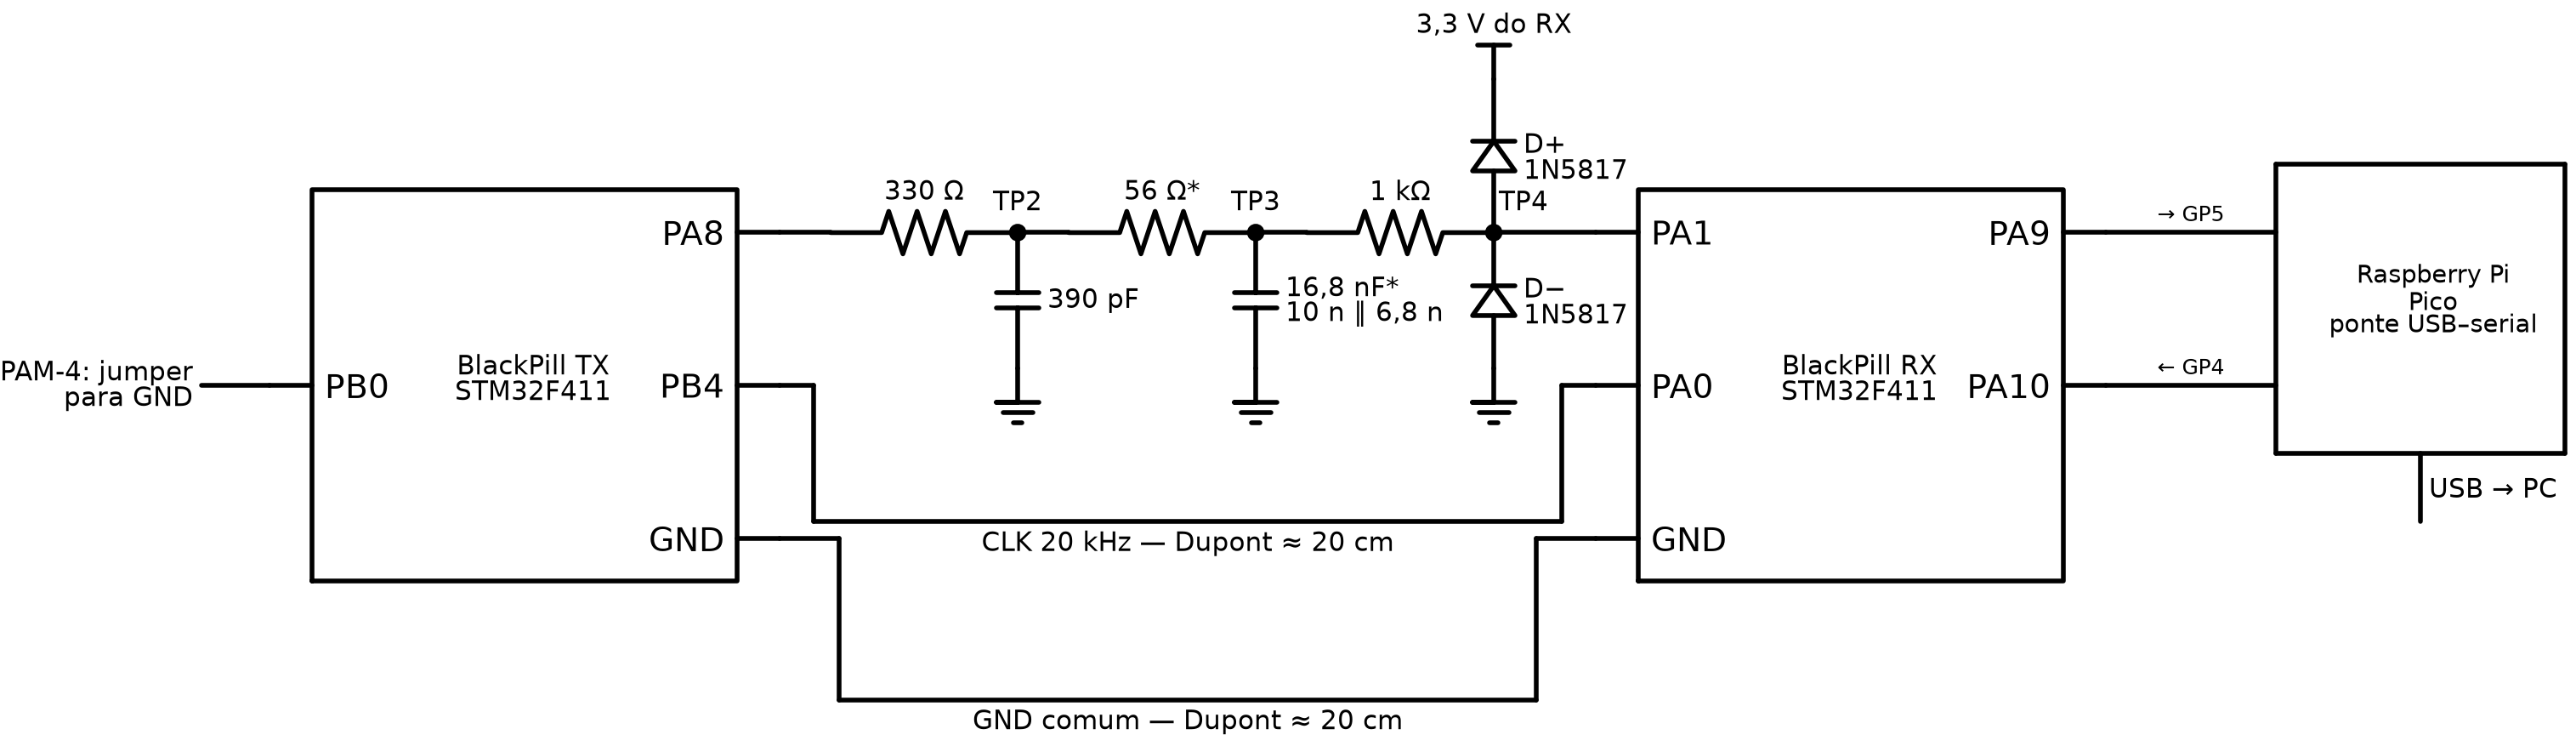
\includegraphics[width=\textwidth]{esquema_montagem.png}
    \caption{Esquema da montagem real. (*) \SI{56}{\ohm} e \SI{16,8}{nF} só no canal 2 (ou
    \SI{33}{nF} no ensaio de verificação). TP1 é o próprio PA8 (PWM bruto).}
    \label{fig:esquema}
\end{figure}

\subsection{Configuração das placas (.ioc)}

Os dois projetos STM32CubeMX (\texttt{TX.ioc} e \texttt{RX.ioc}) seguem o Apêndice A do enunciado:
HSE de \SI{25}{MHz}, PLLM\,=\,25, PLLN\,=\,200, PLLP\,=\,2, SYSCLK de \SI{100}{MHz}, APB1 de
\SI{50}{MHz} e APB2 de \SI{100}{MHz} (TIM1, TIM2 e TIM3 recebem \SI{100}{MHz}), depuração por
\textit{Serial Wire} (PA13/PA14 reservados, PB4 livre). A Tabela~\ref{tab:ioc} resume os periféricos.

\begin{table}[H]
\centering
\caption{Configuração dos periféricos.}
\label{tab:ioc}
\small
\begin{tabularx}{\textwidth}{l l X}
\toprule
Placa & Periférico & Configuração \\
\midrule
TX & TIM1\_CH1 (PA8) & PWM modo 1, PSC\,=\,0, ARR\,=\,2 ($f_{PWM}=\SI{33,333}{MHz}$), preload do CCR1, GPIO muito alta velocidade \\
TX & TIM3\_CH1 (PB4) & PWM modo 1, PSC\,=\,0, ARR\,=\,4999, CCR1\,=\,2500 (CLK de \SI{20}{kHz}, 50\,\%), interrupção de atualização \\
RX & TIM2 & \textit{Slave Reset Mode} por TI1FP1 (PA0, borda de subida), PSC\,=\,0, ARR\,=\,624 (\SI{6,25}{\micro\second}); CH2 \textit{Output Compare} interno, CCR2\,=\,312 (\SI{3,12}{\micro\second}) \\
RX & ADC1\_IN1 (PA1) & 12 bits, \SI{25}{MHz}, 15 ciclos de aquisição, conversão única disparada por TIM2\_CC2 (subida) \\
RX & DMA2 Stream0 Ch0 & circular, 512 posições de 16 bits, interrupções de meia e de transferência completa (256 amostras cada) \\
RX & USART1 (PA9/PA10) & relatório de texto para a ponte USB--serial \\
\bottomrule
\end{tabularx}
\end{table}

\subsection{Firmware}

O código comum (\texttt{pam\_config.h}, \texttt{pam\_frame.c}) contém os parâmetros do enunciado,
o gerador PRBS-15 ($b_{n+15} = b_{n+14}\oplus b_n$, $b_0\ldots b_{14}=1$), o mapeamento Gray e a
sequência do quadro: 140 símbolos de pulso ($20\times$ 0,0,0,A,0,0,0), 256 símbolos de níveis
($32\times$ 0,1,0,0,1,1,0,1 em PAM-2 ou 0,1,0,3,2,3,1,2 em PAM-4), 48 bits de início
(16 bits alternados a partir de 0 e \texttt{0xD391C5A7}) e \num{100000} bits de payload.
O quadro tem \num{100444} símbolos em PAM-2 ($396+48+\num{100000}$) e \num{50420} em PAM-4
($396+24+\num{50000}$).

\textbf{TX.} Antes de iniciar o CLK, TIM1\_CCR1 recebe o nível do símbolo 0. A cada atualização do
TIM3 (subida do CLK), a primeira instrução da ISR escreve em TIM1\_CCR1 o nível já calculado do novo
símbolo, e só depois o nível seguinte é calculado. Ao terminar o último símbolo, o CLK é parado e PA8
volta a \SI{0}{V}.

\textbf{RX.} ADC, DMA e TIM2 são iniciados antes do TX. Na primeira borda do CLK, a ISR registra a
posição de escrita do DMA (512 menos NDTR); a primeira conversão posterior é $a_0[0]$ e as amostras
anteriores são descartadas. Os dados são processados em grupos de oito amostras por símbolo nas
interrupções de meia transferência e de transferência completa do DMA, inclusive quando um grupo
cruza a fronteira entre metades. A cada borda, o firmware confere que o índice absoluto de escrita
avançou exatamente oito amostras; qualquer diferença incrementa \texttt{bordas\_com\_contagem\_errada}.
Ausência de borda por mais de \SI{5}{ms} antes do fim previsto marca \texttt{perda\_CLK}.
Overrun do ADC ou atraso do processamento maior que o buffer também invalidam o quadro.
O treinamento calcula $b_c$, $p_c[k]$ e $E_c$; a calibração escolhe $k^\star$ e os centros, limiares e
margens dos dois detectores, todos congelados antes do início do quadro. O RX confere os 48 bits de
início com os dois detectores e só então compara o payload com a PRBS-15 local.
Ao final, o RX envia por serial os contadores, os parâmetros de treinamento, os 256 símbolos de
calibração e \num{8192} amostras brutas consecutivas do payload (a partir do símbolo \num{1000}),
copiadas para um vetor separado de \SI{16}{kB} durante a recepção.

\subsection{Instrumentação e registro}

O osciloscópio Tektronix TDS2002B (\SI{60}{MHz}) foi controlado pelo PC via USB (USBTMC) por um
script Python que, para cada ensaio, configura as escalas e o disparo, arma o RX pela serial, espera
o RESET do TX e salva a tela, os dados dos dois canais em CSV e o relatório do RX. Os resultados
foram anotados automaticamente em \nolinkurl{entrega/CADERNO_BANCADA.md}. A referência analógica do
ADC foi medida com multímetro: $V_{ref} = \SI{3,297}{V}$, usada na conversão
$V = \text{código}\times V_{ref}/4095$. Todas as análises foram recalculadas no PC a partir das
amostras brutas e conferidas com os valores calculados pelo firmware (mesmo $k^\star$, diferença
máxima em $p_c$ menor que 0,01 código e mesmo $z$ da janela de exemplo).

\subsection{Método da PSD}
\label{sec:metpsd}

Seguindo o enunciado: \num{8192} amostras consecutivas do ADC durante o payload, $f_a =
\SI{160000}{Hz}$, conversão para volts com $V_{ref}$ medido, retirada da média, blocos de
\num{1024} amostras com 50\,\% de sobreposição (15 blocos), janela de Hann e PSD unilateral
$S[f] = 2|\mathrm{FFT}(wx)[f]|^2/(f_a\sum w^2)$ nos bins internos (sem dobrar DC e Nyquist),
seguida da média dos blocos. Resolução: $\Delta f = f_a/N = \SI{156,25}{Hz}$; duração do registro:
\SI{51,2}{ms}. Os valores ``em \SI{5}{kHz}'' e ``em \SI{10}{kHz}'' são a média dos cinco bins em
$\pm\SI{312,5}{Hz}$. Como os blocos começam no mesmo símbolo do payload em todos os ensaios, os bits
são os mesmos e a razão das PSDs entre canais estima $|H(f)|^2$.

% ==================== SEÇÃO 4: RESULTADOS ====================
\section{Resultados e Discussão}

Salvo indicação, os resultados vêm dos quadros válidos listados na Tabela~\ref{tab:logs}, todos
de 03/11/2026, com aquisição válida, sincronismo confirmado e \texttt{calibracao\_ok\,=\,1}.

\begin{table}[H]
\centering
\caption{Quadros usados no relatório (arquivos em \nolinkurl{entrega/logs/}).}
\label{tab:logs}
\small
\begin{tabular}{l c l r r}
\toprule
Canal & PAM & Log do RX & Bordas de CLK & Amostras \\
\midrule
Dupont direto & 2 & \texttt{Dupont\_PAM2\_20261103\_162110} & \num{100444} & \num{803552} \\
Dupont direto & 4 & \texttt{Dupont\_PAM4\_20261103\_162254} & \num{50420} & \num{403360} \\
RC \SI{16,8}{nF} & 2 & \texttt{RC16n8\_PAM2\_20261103\_154922} & \num{100444} & \num{803552} \\
RC \SI{16,8}{nF} & 4 & \texttt{RC16n8\_PAM4\_20261103\_154731} & \num{50420} & \num{403360} \\
RC \SI{33}{nF} & 2 & \texttt{RC33n\_PAM2\_20261103\_161754} & \num{100444} & \num{803552} \\
RC \SI{33}{nF} & 4 & \texttt{RC33n\_PAM4\_20261103\_160314} & \num{50420} & \num{403360} \\
Manga \SI{200}{m} & 2 & \texttt{Manga\_PAM2\_20261103\_165756} & \num{100444} & \num{803552} \\
Manga \SI{200}{m} & 4 & \texttt{Manga\_PAM4\_20261103\_170342} & \num{50420} & \num{403360} \\
\bottomrule
\end{tabular}
\end{table}

\subsection{Verificação do transmissor}

\textbf{CLK.} Medido em PB4: $f = \SI{20,0008}{kHz}$, $T = \SI{49,998}{\micro\second}$, nível
alto de \SI{25,002}{\micro\second} (ciclo de trabalho de 50,0\,\%), \SI{3,56}{V} pico a pico
(Figura~\ref{fig:tx}a).

\textbf{Níveis e ordem Gray.} Os símbolos 140--149 (início da calibração de níveis) foram capturados
em TP2 com o canal Dupont (Figura~\ref{fig:tx}b). A sequência observada foi 0,1,0,3,2,3,1,2,0,1 em
PAM-4 e 0,1,0,0,1,1,0,1,0,1 em PAM-2, como especificado. Os níveis médios medidos em TP2 foram
\SI{-0,011}{V}, \SI{1,017}{V}, \SI{2,142}{V} e \SI{3,377}{V} (PAM-4) e \SI{-0,021}{V} e
\SI{3,380}{V} (PAM-2). Os degraus entre níveis vizinhos não são iguais (1,028; 1,125 e
\SI{1,235}{V}): pulsos de PWM de \SIrange{10}{20}{ns} perdem parte da área nas bordas de subida e
descida do GPIO, o que reduz os níveis intermediários em relação a $V_{DD}/3$ e $2V_{DD}/3$. O nível 3
é o próprio $V_{DD}$ do TX (cerca de \SI{3,38}{V}). O menor degrau (0--1) é o que limita a abertura
do olho PAM-4 nos canais Dupont e RC \SI{16,8}{nF}.

\textbf{Ripple do PWM.} No meio do símbolo 141 (nível 1), TP2 apresenta ripple de
\SI{190}{mV} pico a pico a cerca de \SI{33}{MHz} (média \SI{1,013}{V}; Figura~\ref{fig:tx}c), contra
\SI{150}{mVpp} previstos pelo filtro de um polo. A banda de \SI{60}{MHz} do osciloscópio ainda passa
\SI{33}{MHz}, com alguma atenuação.

\textbf{Alinhamento CLK $\times$ dados.} Com persistência (247 aquisições), as transições de TP2
começam cerca de \SI{0,55}{\micro\second} depois da subida do CLK (Figura~\ref{fig:tx}d), contra os
\SIrange{0,2}{0,4}{\micro\second} previstos para a latência da ISR. Esse atraso é muito menor que o
instante da primeira amostra (\SI{3,12}{\micro\second}) e não afeta a decisão.

\begin{figure}[H]
    \centering
    \begin{subfigure}{0.49\textwidth}\centering
        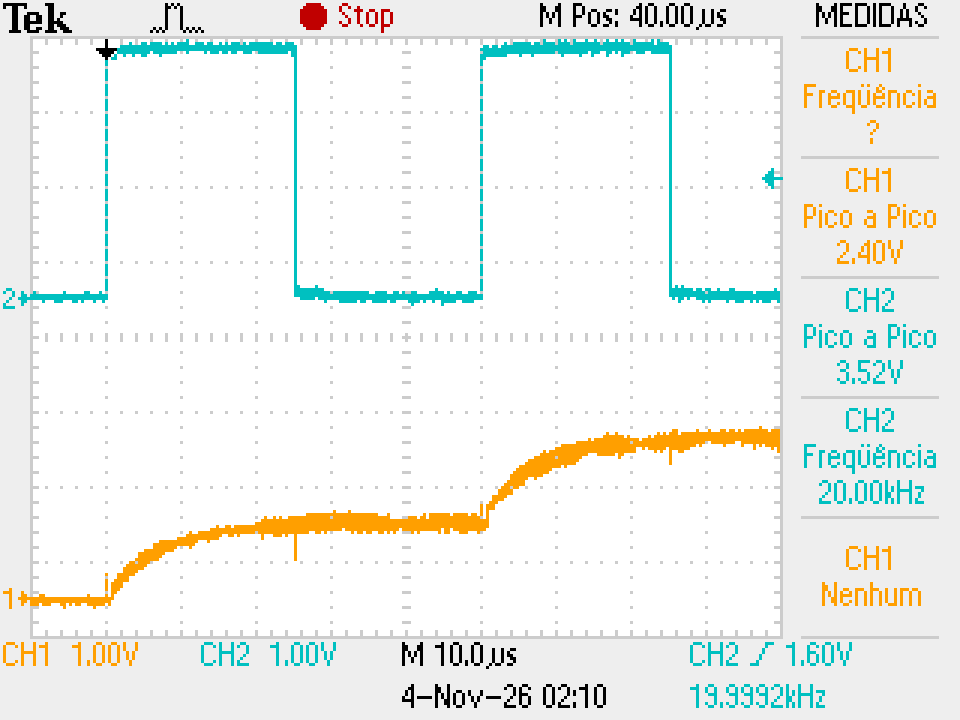
\includegraphics[width=\linewidth]{TX_CLK_50us.png}
        \caption{CLK (CH2) e TP2 (CH1), \SI{10}{\micro\second}/div.}
    \end{subfigure}\hfill
    \begin{subfigure}{0.49\textwidth}\centering
        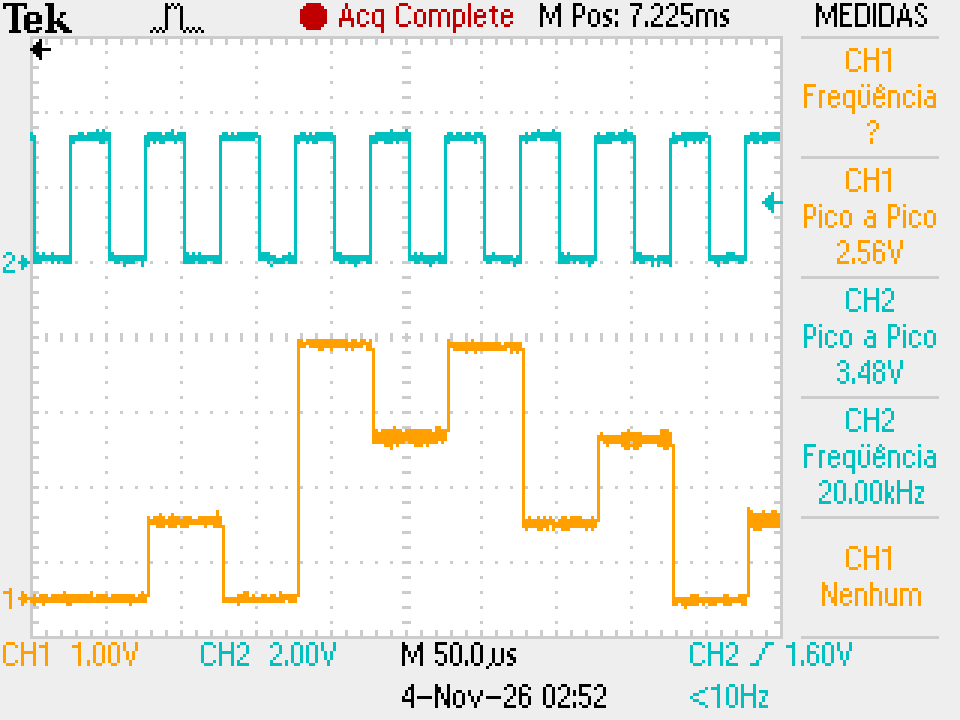
\includegraphics[width=\linewidth]{TX_TP2_PAM4_niveis_gray.png}
        \caption{PAM-4: símbolos 140--149 em TP2 (CH1).}
    \end{subfigure}\\[4pt]
    \begin{subfigure}{0.49\textwidth}\centering
        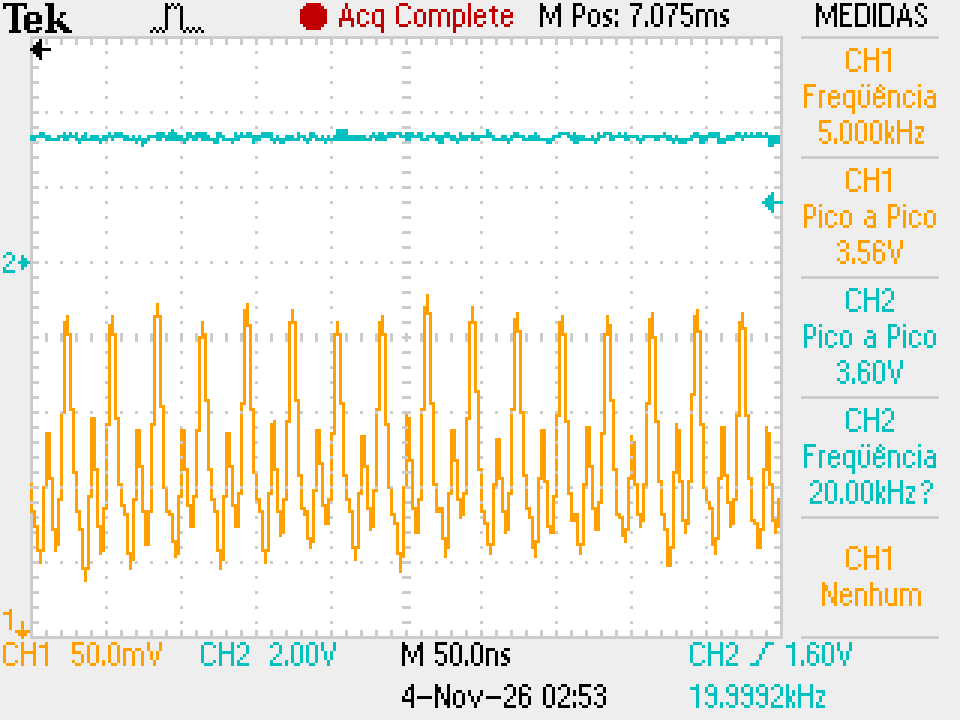
\includegraphics[width=\linewidth]{TX_TP2_PAM4_ripple_PWM.png}
        \caption{Ripple em TP2 no nível 1, \SI{50}{ns}/div, \SI{50}{mV}/div.}
    \end{subfigure}\hfill
    \begin{subfigure}{0.49\textwidth}\centering
        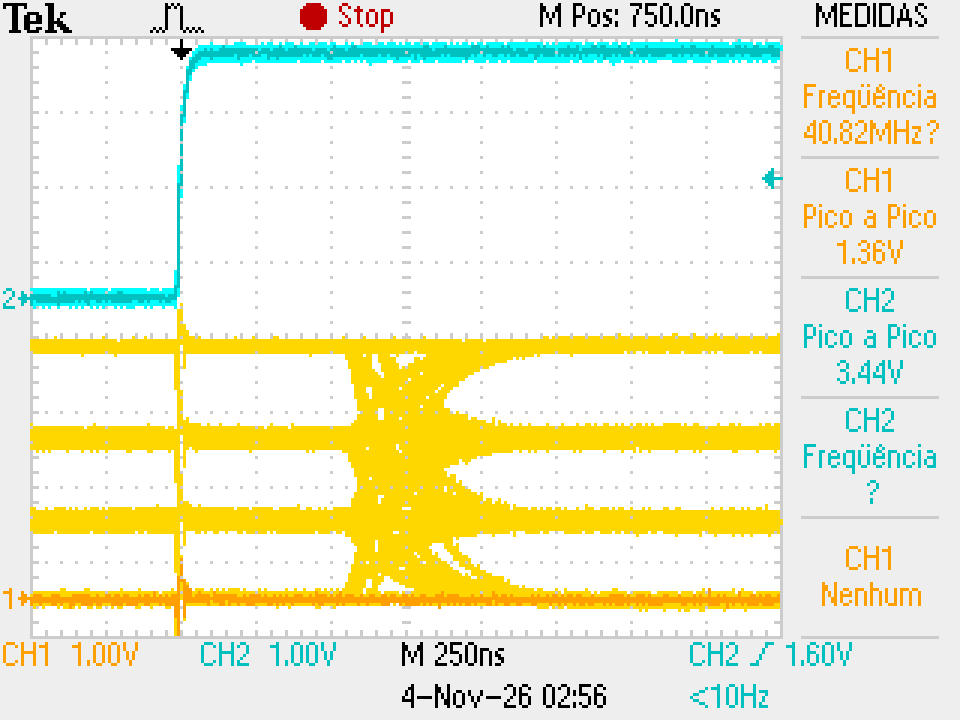
\includegraphics[width=\linewidth]{TX_alinhamento.png}
        \caption{Alinhamento: CLK (CH2) e TP2 (CH1), \SI{250}{ns}/div.}
    \end{subfigure}
    \caption{Verificação do TX (canal Dupont, TP2 com ponta $\times$10). A data na tela é a do
    relógio interno do osciloscópio, que não estava acertado; as capturas são de 03/11/2026.}
    \label{fig:tx}
\end{figure}

\begin{figure}[H]
    \centering
    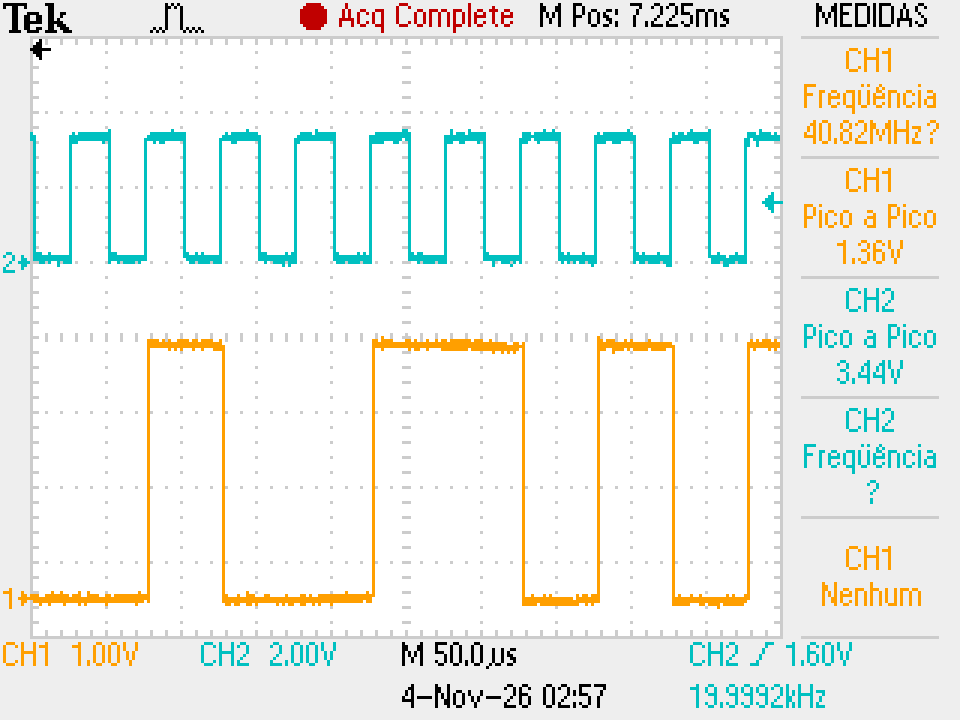
\includegraphics[width=0.55\textwidth]{TX_TP2_PAM2_niveis_gray.png}
    \caption{PAM-2: símbolos 140--149 em TP2 (CH1) e CLK (CH2): 0,1,0,0,1,1,0,1,0,1.}
    \label{fig:tx_pam2}
\end{figure}

\subsection{Verificação do receptor: oito amostras por símbolo}

Em todos os quadros da Tabela~\ref{tab:logs}, o número de bordas de CLK recebidas é igual ao de
símbolos do quadro (\num{100444} ou \num{50420}), o número de amostras processadas é exatamente
$8\times$ o número de bordas e os contadores \texttt{bordas\_com\_contagem\_errada},
\texttt{overrun\_processamento}, \texttt{erro\_ADC\_overrun} e \texttt{perda\_CLK} são nulos.
Como o TIM2 é reiniciado a cada borda e dispara o ADC a cada \SI{6,25}{\micro\second} a partir de
\SI{3,12}{\micro\second}, a taxa de aquisição é $8\times\SI{20}{ksym/s} = \num{160000}$ amostras/s,
e os instantes nominais são $t_k = 3{,}12 + 6{,}25k$\,\si{\micro\second}. As amostras anteriores ao
primeiro CLK (milhões, pois o ADC roda desde o armamento) foram descartadas, como pede o enunciado.

\subsection{Resposta ao degrau e constante de tempo}
\label{sec:tau}

A transição conhecida $0\to A$ do primeiro pulso do treinamento foi capturada com CH1\,=\,TP2 e
CH2\,=\,TP3 (Figura~\ref{fig:degrau}). Em cada captura, $t_0$ é o início da subida em TP2, $V_{63} =
V_0 + 0{,}632(V_f - V_0)$ e $\tau_{med} = t_{63} - t_0$; o tempo de subida $t_{90}-t_{10}$ foi medido
na mesma captura. A Tabela~\ref{tab:tau} compara os valores medidos com os previstos.

\begin{table}[H]
\centering
\caption{Constante de tempo e tempo de subida em TP3 (\si{\micro\second}).}
\label{tab:tau}
\small
\begin{tabular}{l c c c c c c}
\toprule
Canal & PAM & \multicolumn{2}{c}{$\tau$ previsto} & $\tau$ medido & $t_{10-90}$ & $t_{10-90}/2{,}197$ \\
 & & 1 polo & 2 polos & ($t_{63}-t_0$) & medido & \\
\midrule
Dupont (zoom)   & 2 & 0,13 & 0,14 & 0,22 & 0,42 & 0,19 \\
Dupont (zoom)   & 4 & 0,13 & 0,14 & 0,21 & 0,49 & 0,22 \\
RC \SI{16,8}{nF} & 2 & 6,48 & 7,1 & 7,32 & 16,68 & 7,59 \\
RC \SI{16,8}{nF} & 4 & 6,48 & 7,1 & 7,30 & 16,20 & 7,37 \\
RC \SI{33}{nF}   & 2 & 12,74 & 13,9 & 13,20 & 27,10 & 12,34 \\
RC \SI{33}{nF}   & 4 & 12,74 & 13,9 & 13,00 & 27,40 & 12,47 \\
Manga \SI{200}{m} & 2 & -- & -- & 7,3$^\dagger$ & 17,8$^\dagger$ & 8,1$^\dagger$ \\
\bottomrule
\multicolumn{7}{l}{\footnotesize $^\dagger$ indicativo: o cabo é uma linha RC distribuída, não um RC de um polo.}
\end{tabular}
\end{table}

\begin{figure}[H]
    \centering
    \begin{subfigure}{0.49\textwidth}\centering
        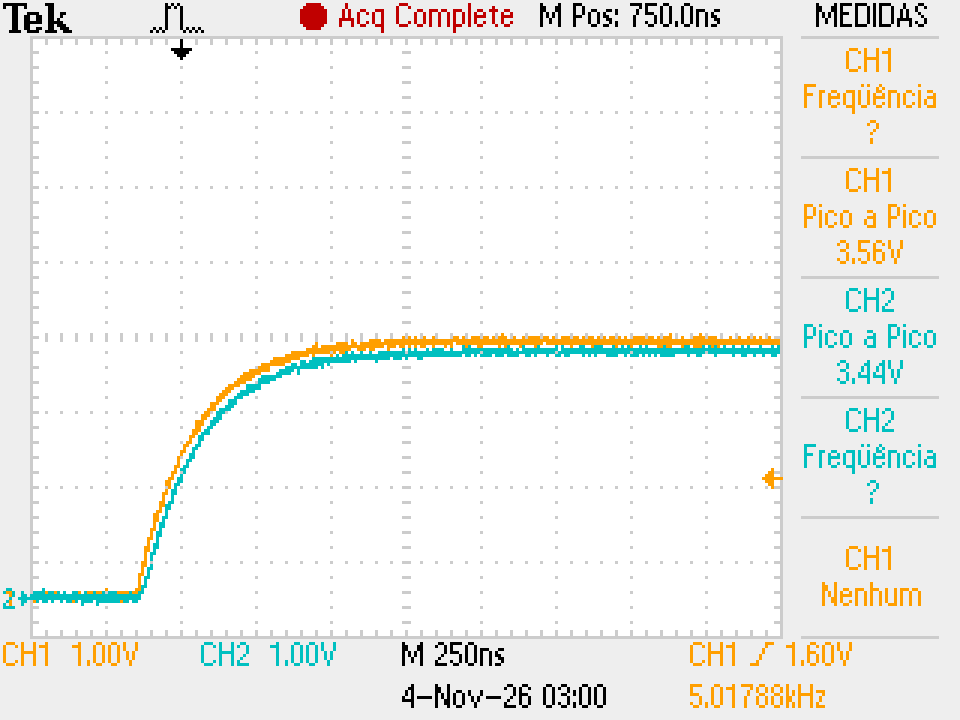
\includegraphics[width=\linewidth]{Dupont_PAM4_TP2_TP3_degrau_zoom.png}
        \caption{Dupont, PAM-4, \SI{250}{ns}/div.}
    \end{subfigure}\hfill
    \begin{subfigure}{0.49\textwidth}\centering
        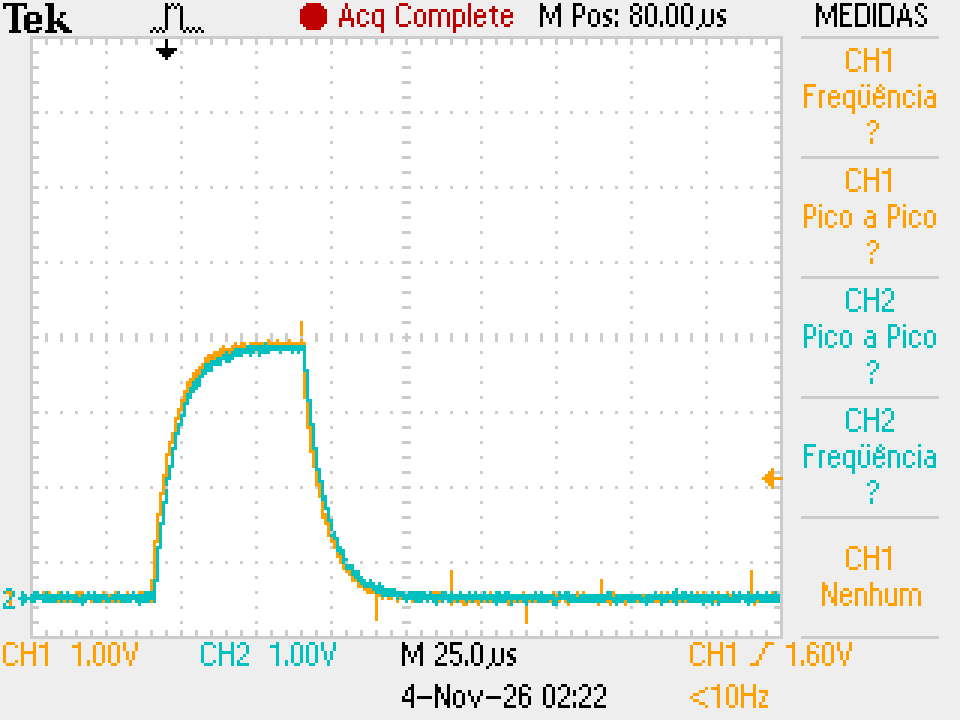
\includegraphics[width=\linewidth]{RC16n8_PAM4_TP2_TP3_degrau.png}
        \caption{RC \SI{16,8}{nF}, PAM-4, \SI{25}{\micro\second}/div.}
    \end{subfigure}\\[4pt]
    \begin{subfigure}{0.49\textwidth}\centering
        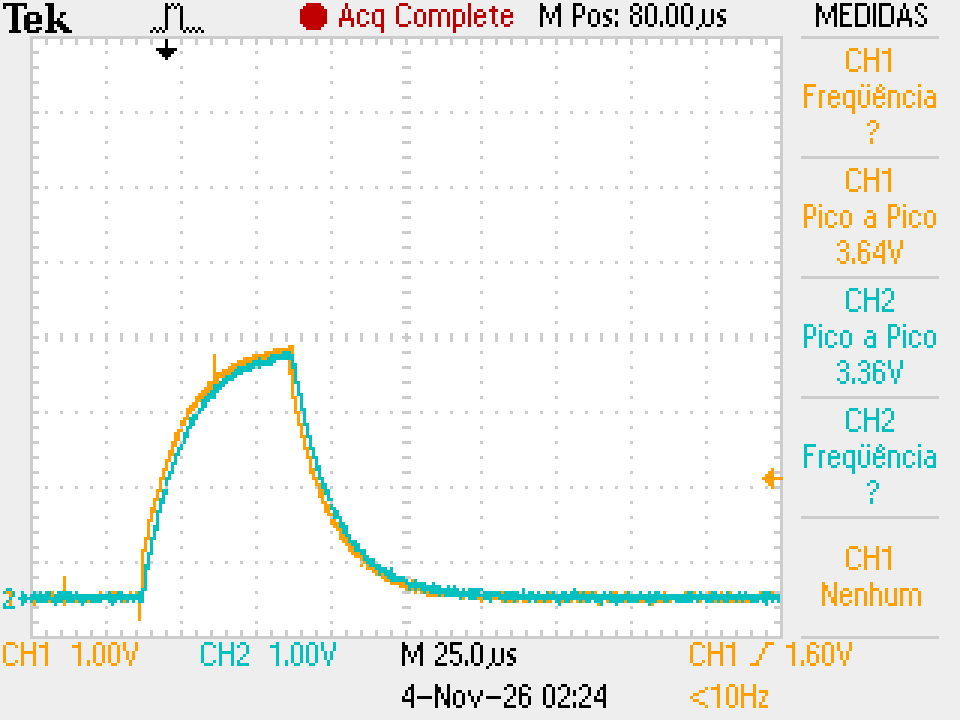
\includegraphics[width=\linewidth]{RC33n_PAM4_TP2_TP3_degrau.png}
        \caption{RC \SI{33}{nF}, PAM-4.}
    \end{subfigure}\hfill
    \begin{subfigure}{0.49\textwidth}\centering
        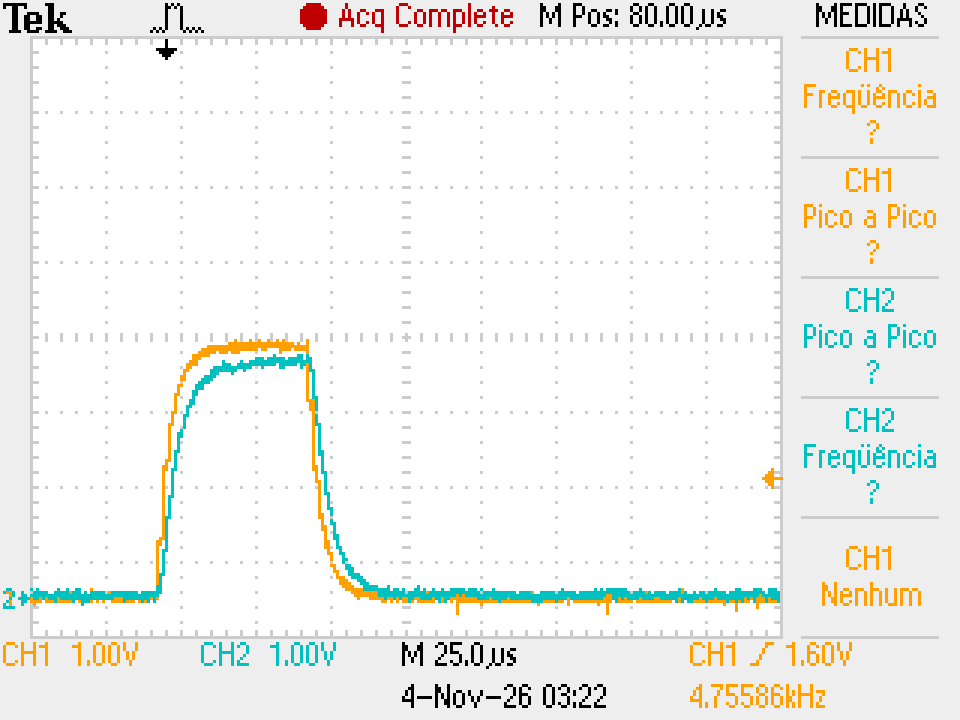
\includegraphics[width=\linewidth]{Manga_PAM2_TP2_TP3_degrau.png}
        \caption{Cabo manga \SI{200}{m}, PAM-2.}
    \end{subfigure}
    \caption{Primeiro pulso $0\to A$ do treinamento: TP2 (CH1, laranja) e TP3 (CH2, azul).}
    \label{fig:degrau}
\end{figure}

\textbf{Canal 2 (\SI{16,8}{nF}).} O valor medido, $\tau = \SI{7,30}{\micro\second}$ (igual em PAM-2
e PAM-4), é 13\,\% maior que o modelo de um polo (\SI{6,48}{\micro\second}) e 3\,\% maior que o
de dois polos (\SI{7,1}{\micro\second}). O tempo de subida medido (\SIrange{16,2}{16,7}{\micro\second})
também é próximo do previsto pelo modelo de dois polos (\SI{15,6}{\micro\second}). A principal causa
verificável da divergência em relação ao modelo de um polo é o filtro do TX: o capacitor de
\SI{390}{pF} e a resistência de saída do GPIO (cerca de \SI{30}{\ohm}) acrescentam um segundo polo e
atrasam o início da subida. Contribuem ainda a tolerância dos capacitores de \SI{10}{nF} e
\SI{6,8}{nF} (tipicamente $\pm 10$\,\%) e a resistência dos fios e contatos da protoboard. A captura
também mostra que, com o canal RC ligado, TP2 não é um degrau ideal: há um salto inicial de cerca de
20\,\% do degrau (divisor resistivo enquanto o capacitor do canal ainda está descarregado) seguido de
uma subida exponencial. Ou seja, o resistor de \SI{330}{\ohm} do TX faz parte do RC do canal, como
supõe o enunciado ao usar $R = 330+56$.

\textbf{Canal 1 (Dupont).} O $\tau$ medido (\SIrange{0,21}{0,30}{\micro\second}, conforme a
captura) é maior que o previsto (\SI{0,13}{\micro\second}). Nessas capturas, a ponta do CH2 em TP3
estava em $\times 1$ (há um offset de cerca de \SI{0,2}{V} na captura PAM-2), e a capacitância de uma
ponta $\times 1$ (da ordem de \SI{100}{pF}) soma-se aos \SI{390}{pF}, além de reduzir a banda da
medição. Em qualquer caso, a resposta do canal Dupont termina em menos de \SI{1}{\micro\second},
bem antes da primeira amostra.

\textbf{Troca para \SI{33}{nF}.} O $\tau$ medido de \SIrange{13,0}{13,2}{\micro\second} fica entre os
modelos de um polo (\SI{12,74}{\micro\second}) e de dois polos (\SI{13,9}{\micro\second}), e o tempo
de subida dobra para \SIrange{27,1}{27,4}{\micro\second} (previsto cerca de \SI{28}{\micro\second}).
Como $e^{-T_s/\tau}$ passa de \num{0.1}\,\% para cerca de 2\,\%, a ISI deixa de ser desprezível: o
resíduo em TP3 no fim do primeiro zero depois de A foi de \SI{+120}{mV} (previsto \SI{68}{mV};
resolução do osciloscópio de cerca de \SI{40}{mV} a \SI{1}{V/div}), contra \SI{+22}{mV} com
\SI{16,8}{nF}.

\subsection{Diagramas de olho e escolha de $k^\star$}

A posição da amostra única foi fixada pelo firmware a partir dos 256 símbolos de calibração (menor
separação entre níveis vizinhos em cada $k$; maior delas; menor $k$ em caso de empate). A
Tabela~\ref{tab:olho} mostra a abertura vertical do olho em cada $k$, calculada com \num{1024}
símbolos do payload (menor diferença entre o mínimo do nível superior e o máximo do inferior).
Valores negativos indicam que as faixas de níveis vizinhos se cruzam nesse instante.

\begin{table}[H]
\centering
\caption{Abertura vertical do olho (V) em cada posição $k$ ($t_k = 3{,}12+6{,}25k$ \si{\micro\second}),
e $k^\star$ escolhido pela calibração.}
\label{tab:olho}
\footnotesize
\setlength{\tabcolsep}{4pt}
\begin{tabular}{l c r r r r r r r r c}
\toprule
Canal & PAM & $k=0$ & 1 & 2 & 3 & 4 & 5 & 6 & 7 & $k^\star$ ($t$) \\
\midrule
Dupont & 2 & 3,291 & 3,291 & 3,290 & 3,287 & 3,289 & 3,291 & 3,288 & 3,286 & 1 (\SI{9,37}{\micro\second}) \\
Dupont & 4 & 0,970 & 0,965 & 0,968 & 0,966 & 0,967 & 0,969 & 0,964 & 0,965 & 7 (\SI{46,87}{\micro\second}) \\
RC 16,8 nF & 2 & $-$0,916 & 1,539 & 2,559 & 2,977 & 3,154 & 3,233 & 3,264 & 3,273 & 7 (\SI{46,87}{\micro\second}) \\
RC 16,8 nF & 4 & $-$1,756 & $-$0,159 & 0,503 & 0,779 & 0,895 & 0,947 & 0,968 & 0,979 & 7 (\SI{46,87}{\micro\second}) \\
RC 33 nF & 2 & $-$2,411 & $-$0,406 & 0,900 & 1,746 & 2,295 & 2,623 & 2,854 & 2,989 & 7 (\SI{46,87}{\micro\second}) \\
RC 33 nF & 4 & $-$2,408 & $-$1,165 & $-$0,382 & 0,117 & 0,432 & 0,629 & 0,759 & 0,838 & 7 (\SI{46,87}{\micro\second}) \\
Manga & 2 & 0,536 & 2,597 & 3,062 & 3,179 & 3,221 & 3,226 & 3,254 & 3,262 & 7 (\SI{46,87}{\micro\second}) \\
Manga & 4 & $-$0,808 & 0,528 & 0,838 & 0,923 & 0,944 & 0,958 & 0,958 & 0,970 & 7 (\SI{46,87}{\micro\second}) \\
\bottomrule
\end{tabular}
\end{table}

No canal Dupont, a resposta é tão rápida que todas as posições são praticamente equivalentes: as
separações de calibração diferem por poucos códigos (por exemplo, \numrange{4085}{4089} códigos em
PAM-2), e o $k^\star$ escolhido ($k=1$ em PAM-2, $k=7$ em PAM-4) é decidido por diferenças da ordem do
ruído. Nos canais RC e no cabo manga, a abertura cresce monotonicamente com $k$ e o melhor instante é
o último, $k^\star = 7$ (\SI{46,87}{\micro\second} após a borda), quando a exponencial está mais perto
do valor final. Com \SI{33}{nF}, o olho PAM-4 só abre a partir de $k=3$.

Em PAM-4, o par de níveis mais próximo foi o 0--1 (bits Gray 00/01) em todos os canais para a
amostra única, consequência do menor degrau de nível gerado pelo TX (\SI{1,028}{V}). As aberturas
em $k^\star$ foram \SI{0,965}{V} (Dupont), \SI{0,979}{V} (RC \SI{16,8}{nF}) e \SI{0,838}{V}
(RC \SI{33}{nF}). Em PAM-2 foram 3,291; 3,273 e \SI{2,989}{V}.

A Figura~\ref{fig:olhos} mostra os olhos em TP3 no osciloscópio (CH1\,=\,TP3, CH2\,=\,CLK, disparo
na subida do CLK, persistência infinita), com a linha vertical em $t_{k^\star}$. A Figura~\ref{fig:rx}
mostra, para cada condição obrigatória, a sobreposição das próprias amostras do RX (painel superior
direito), que é a evidência usada para a abertura numérica. As capturas de olho PAM-2 do osciloscópio
salvas em \nolinkurl{entrega/capturas/} contêm traços residuais da persistência de aquisições
anteriores (por exemplo, uma curva exponencial no olho do canal Dupont); por isso, para PAM-2, o olho
apresentado é o das amostras do RX.

\begin{figure}[H]
    \centering
    \begin{subfigure}{0.49\textwidth}\centering
        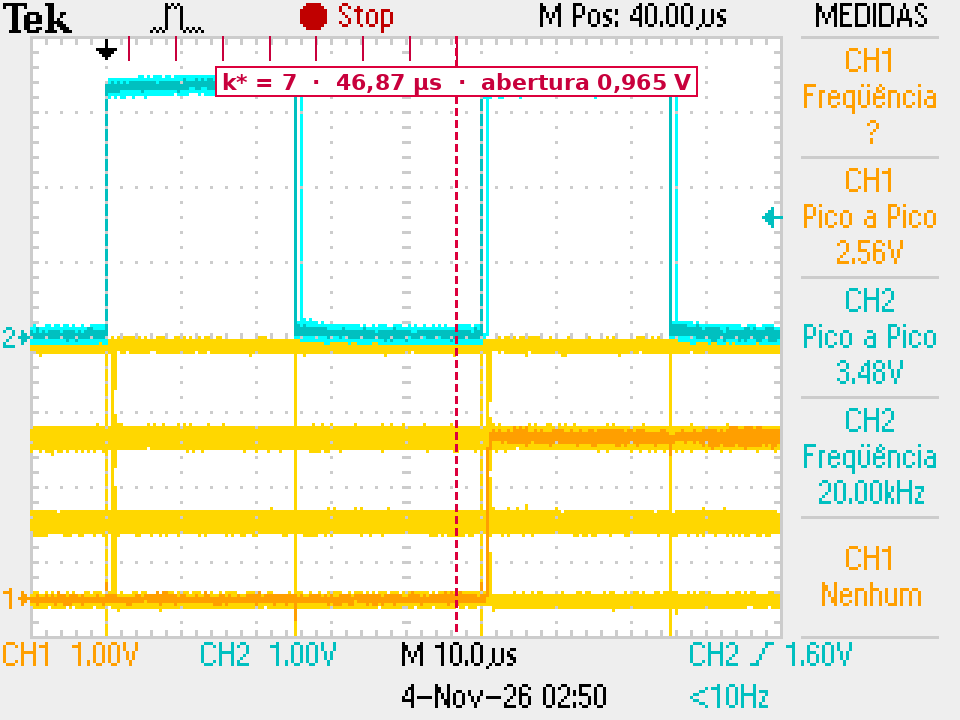
\includegraphics[width=\linewidth]{olho_osc_Dupont_PAM4.png}
        \caption{Dupont, PAM-4.}
    \end{subfigure}\hfill
    \begin{subfigure}{0.49\textwidth}\centering
        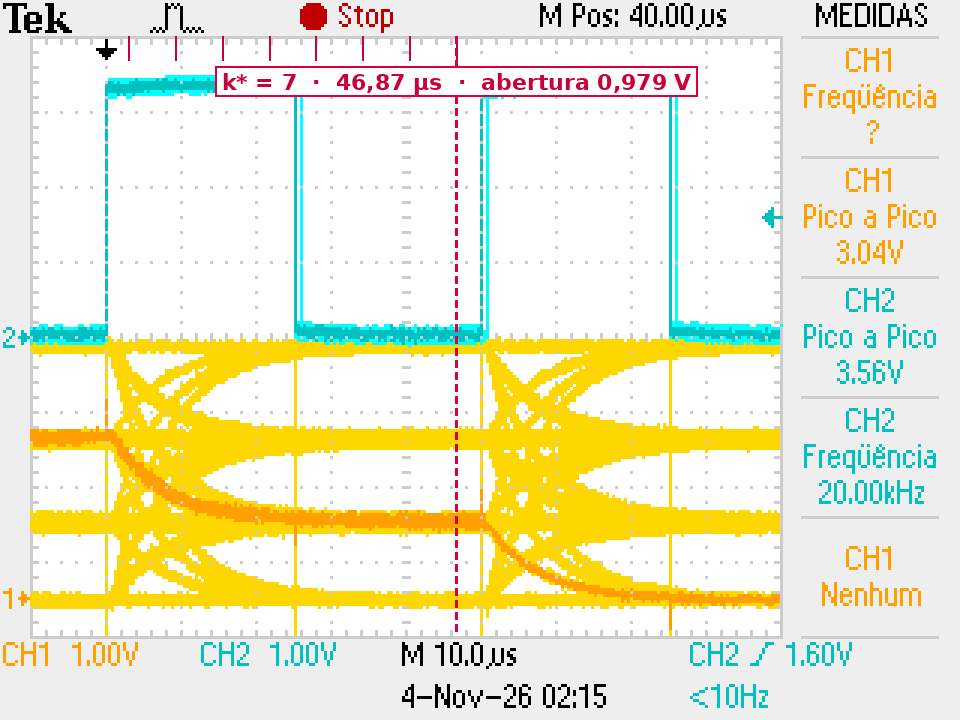
\includegraphics[width=\linewidth]{olho_osc_RC16n8_PAM4.png}
        \caption{RC \SI{16,8}{nF}, PAM-4.}
    \end{subfigure}\\[4pt]
    \begin{subfigure}{0.49\textwidth}\centering
        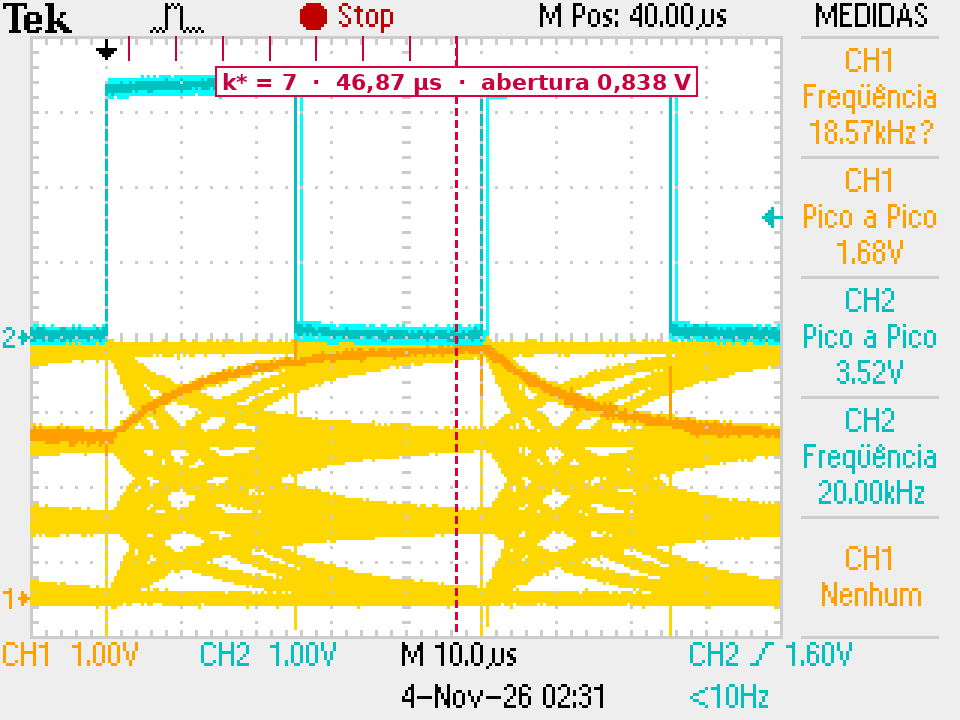
\includegraphics[width=\linewidth]{olho_osc_RC33n_PAM4.png}
        \caption{RC \SI{33}{nF}, PAM-4.}
    \end{subfigure}\hfill
    \begin{subfigure}{0.49\textwidth}\centering
        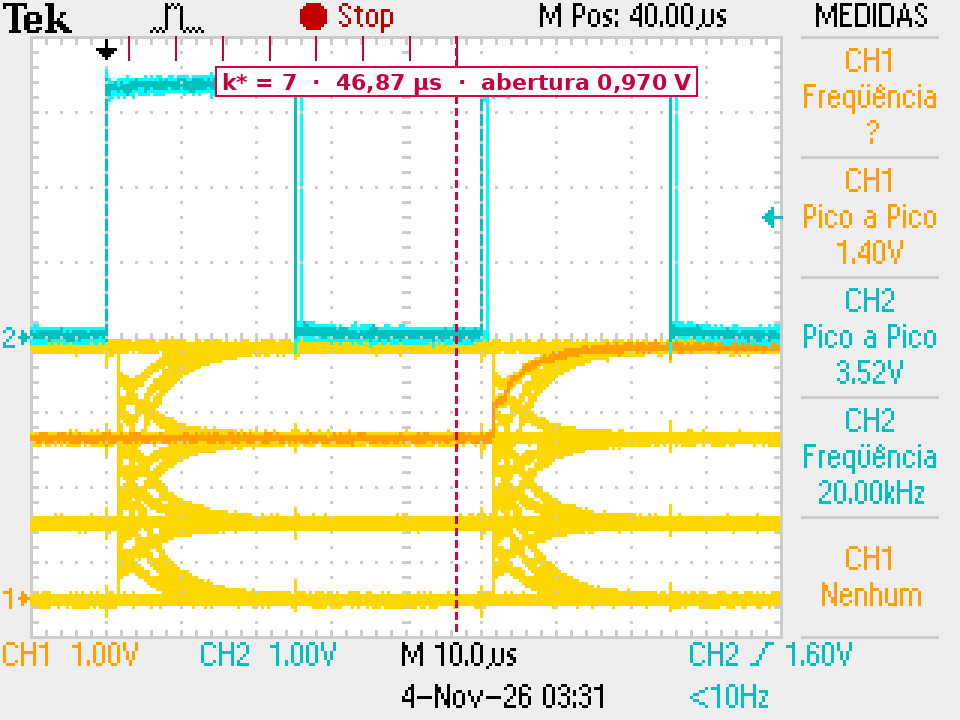
\includegraphics[width=\linewidth]{olho_osc_Manga_PAM4.png}
        \caption{Cabo manga \SI{200}{m}, PAM-4.}
    \end{subfigure}
    \caption{Olho em TP3 no osciloscópio (\SI{10}{\micro\second}/div, \SI{1}{V/div}); linha
    tracejada em $k^\star=7$ (\SI{46,87}{\micro\second}); abertura anotada calculada pelo RX.}
    \label{fig:olhos}
\end{figure}

\begin{figure}[p]
    \centering
    \begin{subfigure}{\textwidth}\centering
        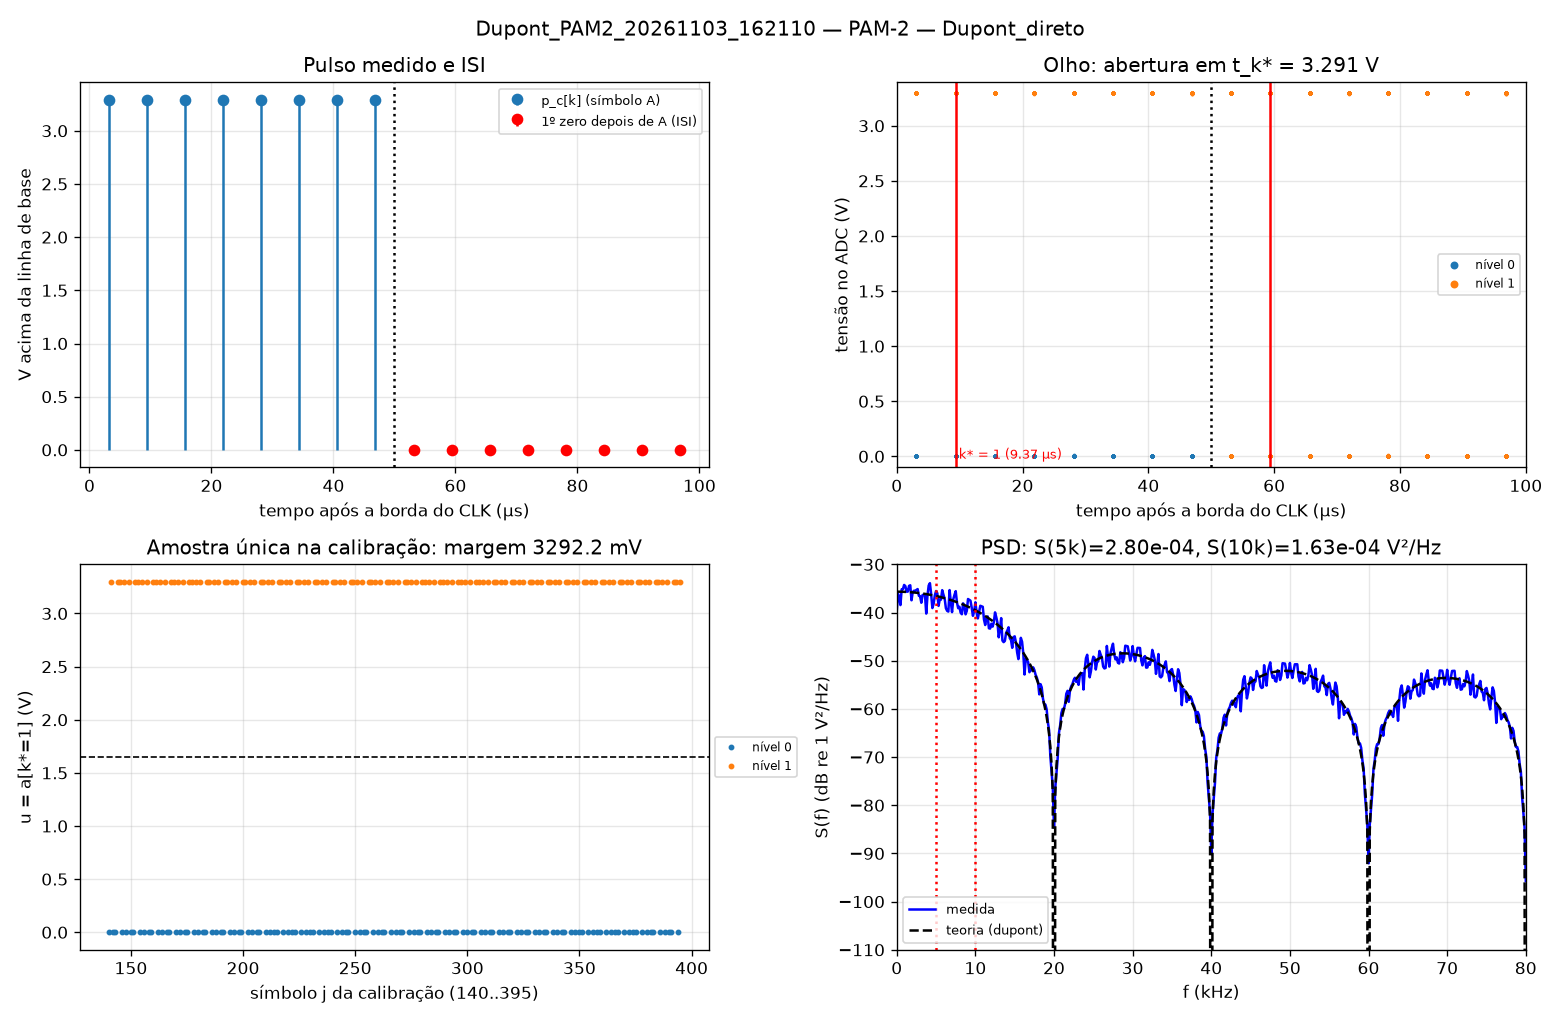
\includegraphics[width=0.92\linewidth]{rx_Dupont_PAM2.png}
        \caption{Dupont, PAM-2.}
    \end{subfigure}\\[2pt]
    \begin{subfigure}{\textwidth}\centering
        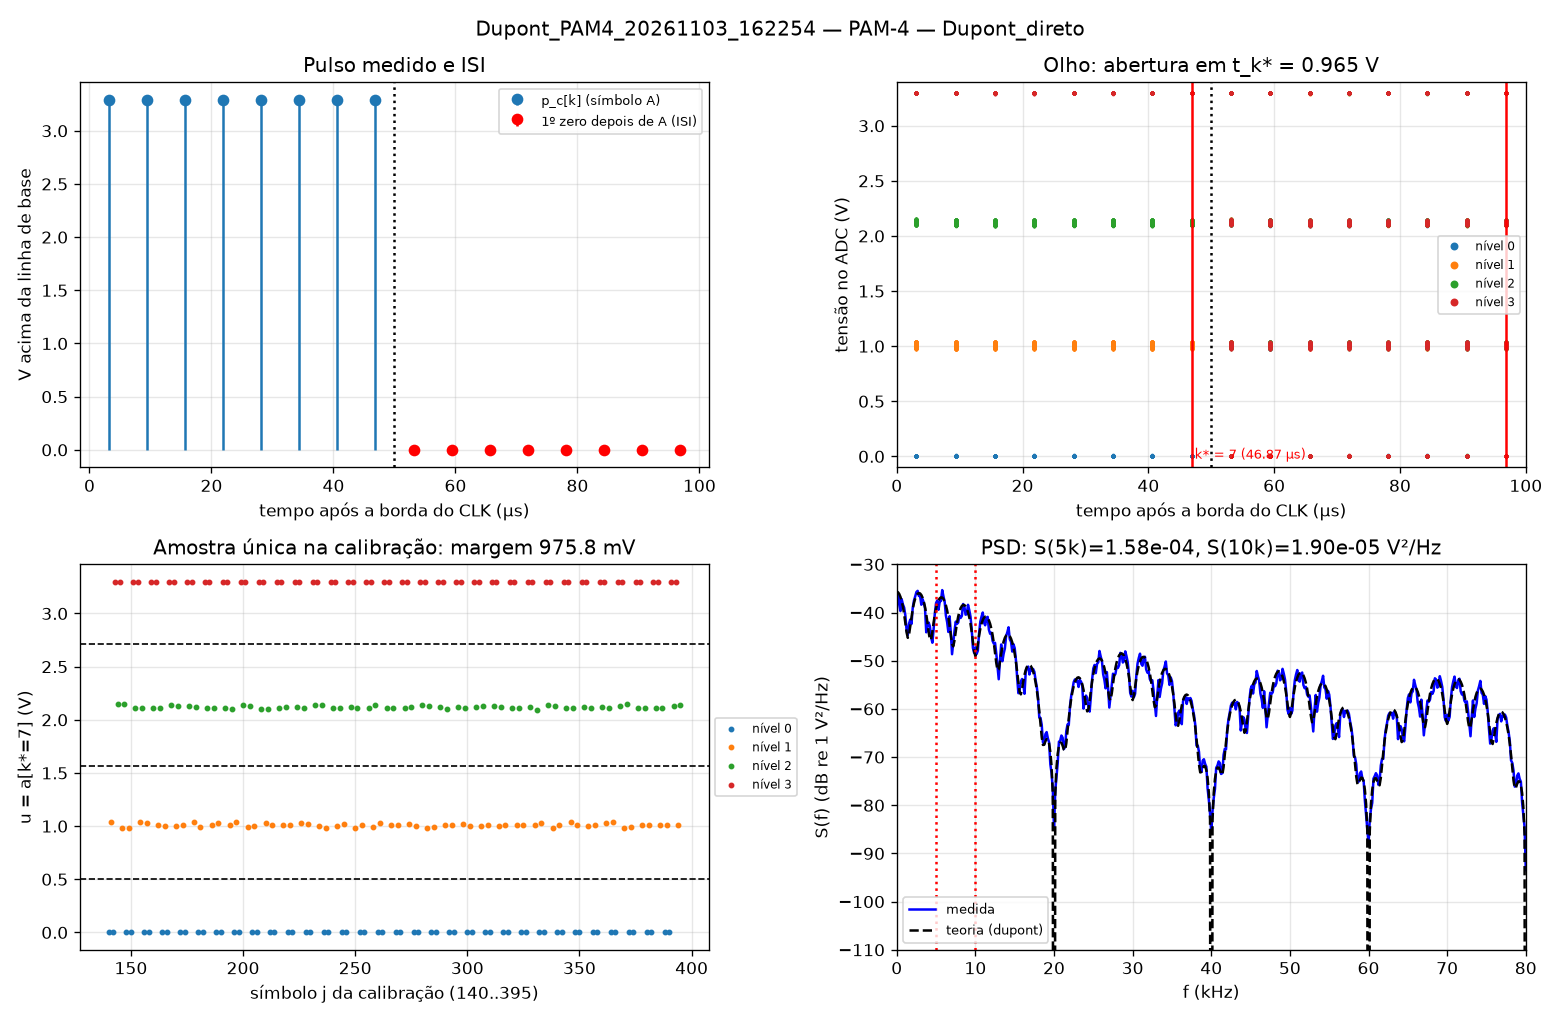
\includegraphics[width=0.92\linewidth]{rx_Dupont_PAM4.png}
        \caption{Dupont, PAM-4.}
    \end{subfigure}
    \caption{Análise dos quadros do canal Dupont a partir das amostras do RX: pulso medido $p_c[k]$
    e ISI (sup. esq.), olho das amostras com $k^\star$ (sup. dir.), amostra única na calibração com
    limiares (inf. esq.) e PSD medida $\times$ teórica (inf. dir.).}
    \label{fig:rx}
\end{figure}

\begin{figure}[p]
    \centering
    \begin{subfigure}{\textwidth}\centering
        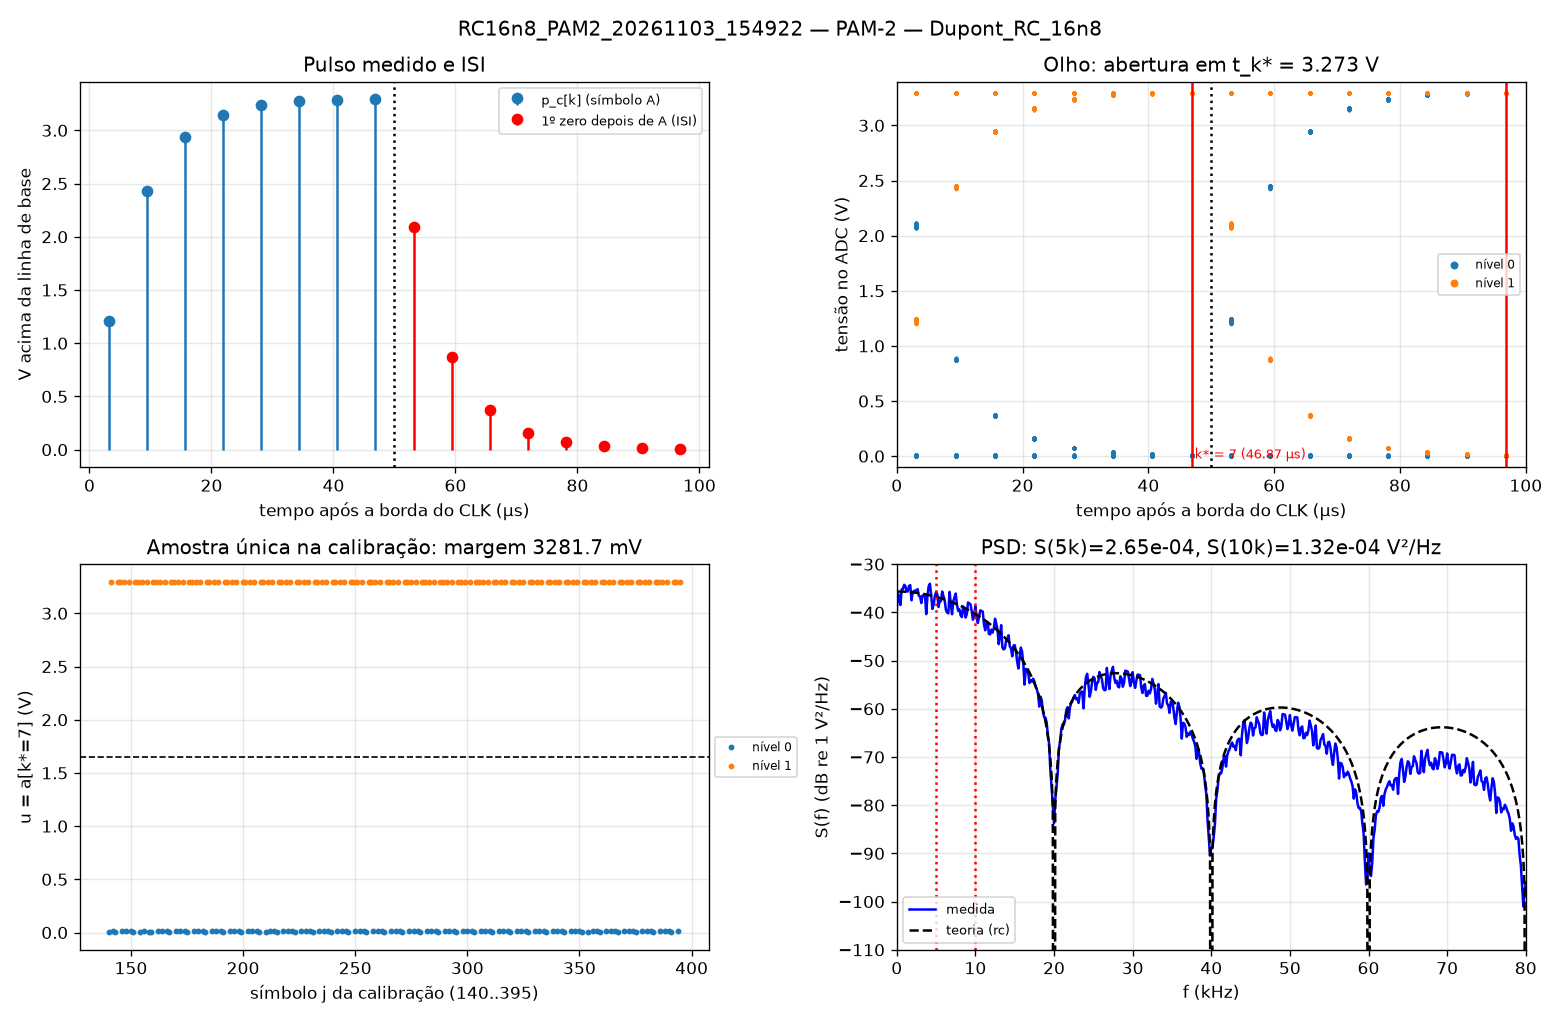
\includegraphics[width=0.92\linewidth]{rx_RC16n8_PAM2.png}
        \caption{RC \SI{16,8}{nF}, PAM-2.}
    \end{subfigure}\\[2pt]
    \begin{subfigure}{\textwidth}\centering
        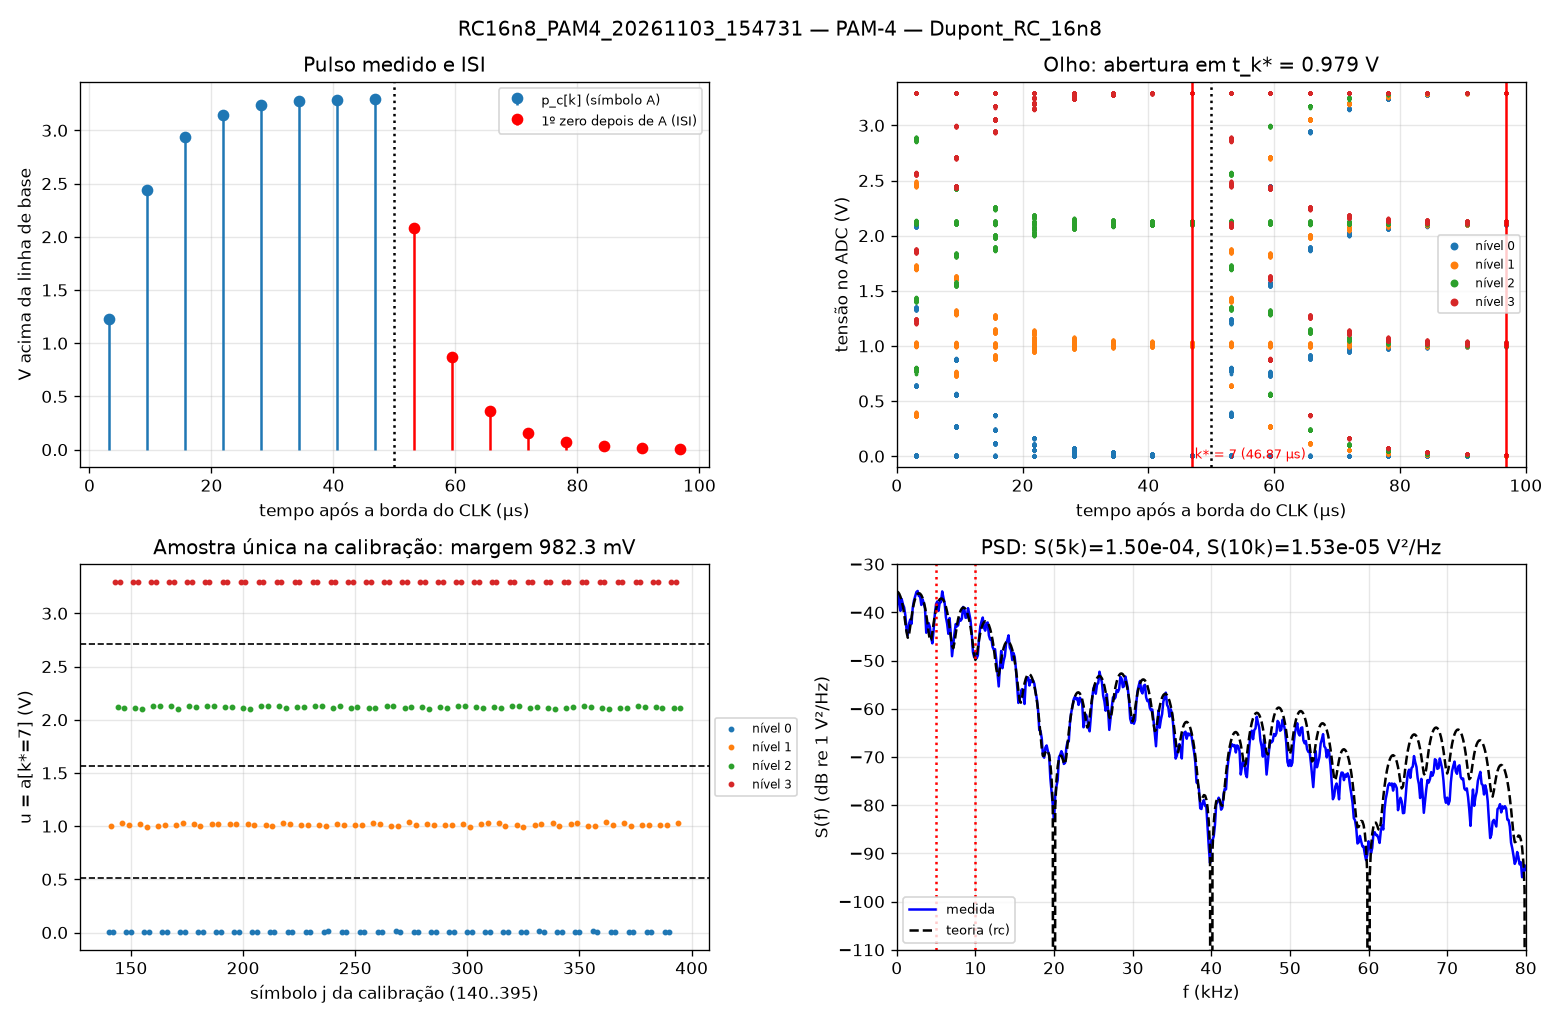
\includegraphics[width=0.92\linewidth]{rx_RC16n8_PAM4.png}
        \caption{RC \SI{16,8}{nF}, PAM-4.}
    \end{subfigure}
    \caption{Análise dos quadros do canal RC \SI{16,8}{nF} (mesma organização da Figura~\ref{fig:rx}).}
    \label{fig:rx_rc}
\end{figure}

\subsection{Densidade espectral de potência}

A Tabela~\ref{tab:psd} apresenta a PSD medida em \SI{5}{kHz} e \SI{10}{kHz}, e a
Figura~\ref{fig:psd} compara os canais na mesma escala. Os valores do canal Dupont concordam com a
expressão teórica da Seção~\ref{sec:teopsd} com $V_{ref}$ medido (por exemplo, PAM-2 em \SI{5}{kHz}:
\SI{2,10e-4}{V^2/Hz} medido e \SI{2,21e-4}{V^2/Hz} previsto).

\begin{table}[H]
\centering
\caption{PSD medida (\si{V^2/Hz}, média de 5 bins) e razão em relação ao canal Dupont com a mesma modulação.}
\label{tab:psd}
\small
\begin{tabular}{l c c c c c c c}
\toprule
Canal & PAM & $S(\SI{5}{kHz})$ & $S(\SI{10}{kHz})$ & \multicolumn{2}{c}{Razão medida} & \multicolumn{2}{c}{$|H|^2$ 2 polos} \\
 & & & & \SI{5}{kHz} & \SI{10}{kHz} & \SI{5}{kHz} & \SI{10}{kHz} \\
\midrule
Dupont & 2 & \num{2.101e-4} & \num{1.062e-4} & 1 & 1 & -- & -- \\
Dupont & 4 & \num{1.187e-4} & \num{1.639e-5} & 1 & 1 & -- & -- \\
RC 16,8 nF & 2 & \num{1.985e-4} & \num{8.616e-5} & 0,944 & 0,812 & 0,952 & 0,834 \\
RC 16,8 nF & 4 & \num{1.123e-4} & \num{1.325e-5} & 0,946 & 0,808 & 0,952 & 0,834 \\
RC 33 nF & 2 & \num{1.725e-4} & \num{5.751e-5} & 0,821 & 0,542 & 0,841 & 0,569 \\
RC 33 nF & 4 & \num{9.904e-5} & \num{9.112e-6} & 0,834 & 0,556 & 0,841 & 0,569 \\
Manga & 2 & \num{2.026e-4} & \num{9.496e-5} & 0,964 & 0,894 & -- & -- \\
Manga & 4 & \num{1.145e-4} & \num{1.459e-5} & 0,965 & 0,890 & -- & -- \\
\bottomrule
\end{tabular}
\end{table}

\begin{figure}[H]
    \centering
    \begin{subfigure}{\textwidth}\centering
        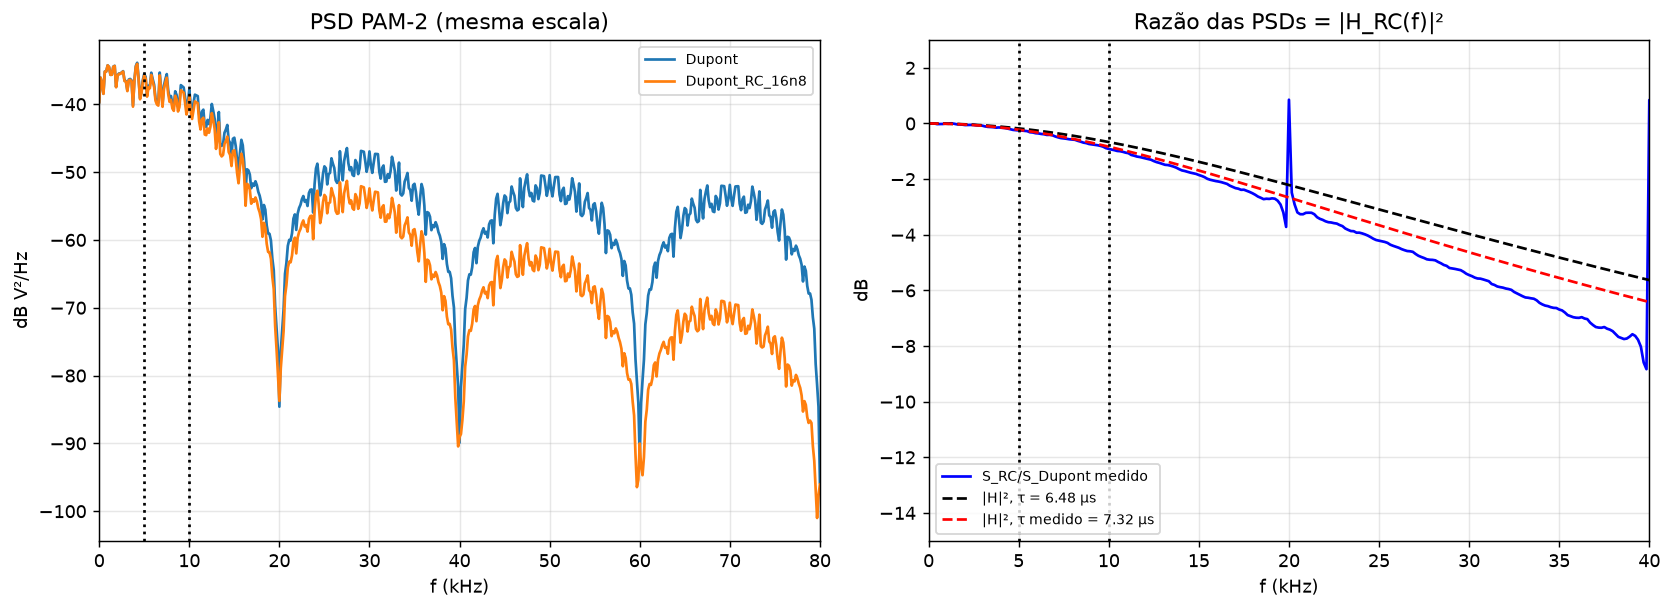
\includegraphics[width=0.95\linewidth]{psd_RC16n8_PAM2.png}
        \caption{PAM-2: Dupont $\times$ RC \SI{16,8}{nF}.}
    \end{subfigure}\\[2pt]
    \begin{subfigure}{\textwidth}\centering
        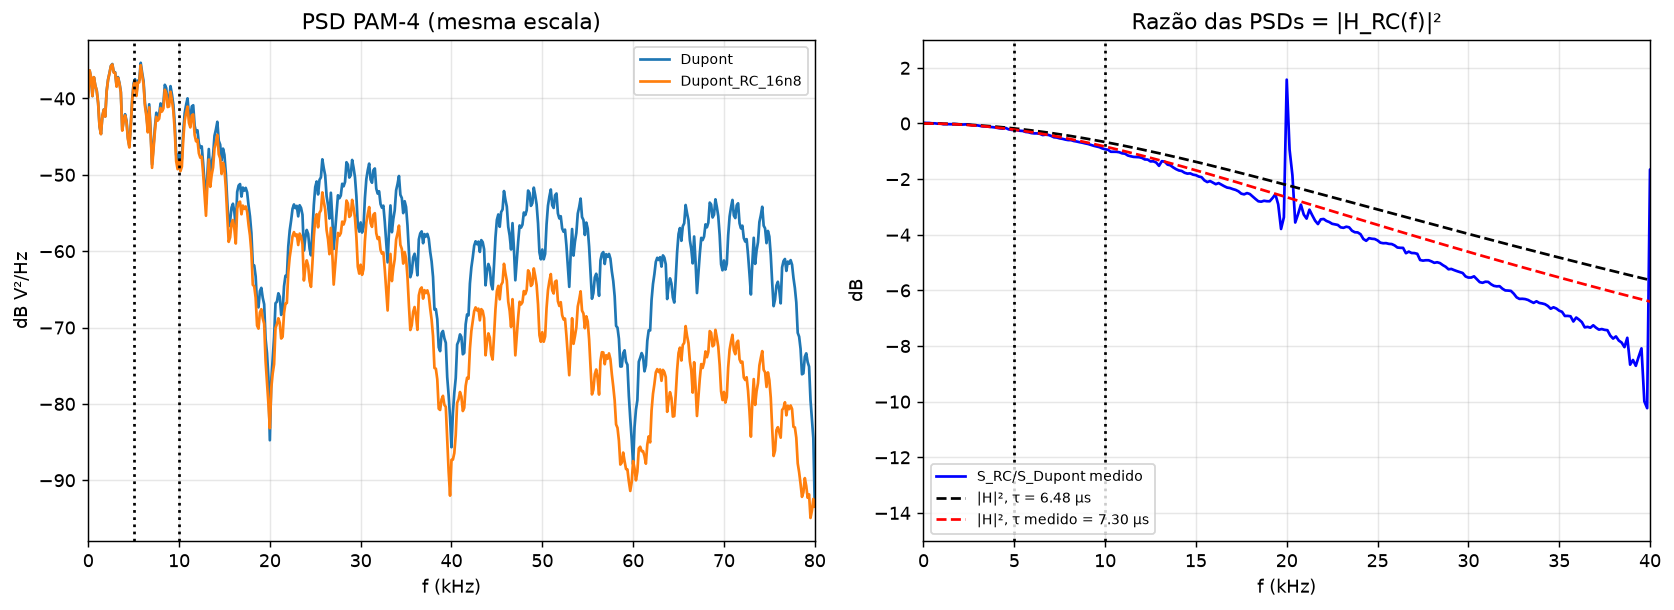
\includegraphics[width=0.95\linewidth]{psd_RC16n8_PAM4.png}
        \caption{PAM-4: Dupont $\times$ RC \SI{16,8}{nF}.}
    \end{subfigure}
    \caption{Esquerda: PSDs na mesma escala (dB re \SI{1}{V^2/Hz}); direita: razão
    $S_{RC}/S_{Dupont}$ comparada com $|H(f)|^2$ de um polo com $\tau$ nominal e com $\tau$ medido.
    Os picos isolados em \SI{20}{kHz} e \SI{40}{kHz} da razão são divisões entre valores próximos de
    zero nos nulos da PSD (múltiplos de $R_s$), e não ganho do canal.}
    \label{fig:psd}
\end{figure}

\textbf{Razão entre as frequências.} No canal Dupont, $S(\SI{10}{kHz})/S(\SI{5}{kHz}) = 0{,}505$
em PAM-2, próximo do valor teórico $\mathrm{sinc}^2(0{,}5)/\mathrm{sinc}^2(0{,}25) = 0{,}405/0{,}811
= 0{,}50$. Em PAM-4 a razão é bem menor (0,138 medida; 0,10 prevista). Ao agrupar em pares os
bits da PRBS-15, a recorrência $b_{n+15}=b_{n+14}\oplus b_n$ liga bits separados por 14 posições,
ou seja, símbolos PAM-4 separados por 7 posições. Os símbolos deixam de ser independentes e a PSD
ganha um fator proporcional a $5+4\cos(2\pi f\cdot 7T_s)$, que vale 5 em \SI{5}{kHz} e 1 em
\SI{10}{kHz} (curva teórica na Figura~\ref{fig:rx}). Por isso, a comparação entre canais deve ser
feita com a mesma modulação, como na Tabela~\ref{tab:psd}.

\textbf{Efeito do canal.} A razão RC/Dupont independe da modulação (0,944 e 0,946 em \SI{5}{kHz};
0,812 e 0,808 em \SI{10}{kHz}): ela caracteriza o canal, e não o sinal, como esperado para um sistema
LIT. Os valores medidos ficam de 1\,\% a 3\,\% abaixo do modelo de dois polos, coerente com um $\tau$
real um pouco maior que o modelo (\SI{7,30}{\micro\second} medidos contra \SI{7,1}{\micro\second}).
Com $\tau = \SI{7,30}{\micro\second}$, um polo dá 0,950 e 0,826, que concordam com as medidas dentro
de 2\,\%. Com \SI{33}{nF}, a atenuação em \SI{10}{kHz} passa a 0,54--0,56 (cerca de \SI{-2,6}{dB}),
e a componente de \SI{10}{kHz} perde quase metade da potência. A redução das componentes de frequência
mais alta é a mesma informação que o tempo de subida maior mostra no domínio do tempo e que aparece no
olho como ISI.

\textbf{Aliasing do PWM.} A frequência de Nyquist do ADC é $f_a/2 = \SI{80}{kHz}$. O ripple de
\SI{33,333}{MHz} rebate para $33\,333\,333 - 208\times\num{160000} = \SI{53,3}{kHz}$. Nas oito PSDs
medidas, o bin mais próximo de \SI{53,3}{kHz} fica de 3 a \SI{4}{dB} acima dos vizinhos, um indício
fraco de resíduo de PWM rebatido, cerca de \SI{20}{dB} abaixo do pico da PSD. Como não há filtro
antialiasing além do RC do TX e da proteção, componentes acima de \SI{80}{kHz} podem aparecer nas
amostras.

\textbf{Osciloscópio $\times$ ADC.} O nível 3 do TX em TP2 é de cerca de \SI{3,38}{V}, acima de
$V_{ref} = \SI{3,297}{V}$ do RX. O ADC satura em \num{4095} códigos para esse nível (centro do nível 3
igual a \num{4095} nos canais Dupont e RC \SI{16,8}{nF}), enquanto o osciloscópio mostra o valor
completo. A saturação é a razão de os pesos $p_c[k]$ do canal Dupont serem praticamente constantes
(\num{4091} códigos) e de a abertura PAM-2 ser limitada a cerca de $V_{ref}$.

\subsection{Filtro casado: treinamento, janela real e comparação com a amostra única}

A Tabela~\ref{tab:pc} mostra a linha de base $b_c$ e os oito pesos $p_c[k]$ obtidos no treinamento
de cada condição (em códigos do ADC).

\begin{table}[H]
\centering
\caption{Linha de base e coeficientes do filtro casado (códigos do ADC).}
\label{tab:pc}
\footnotesize
\setlength{\tabcolsep}{3.5pt}
\begin{tabular}{l c r r r r r r r r r r}
\toprule
Canal & PAM & $b_c$ & $p_c[0]$ & $p_c[1]$ & $p_c[2]$ & $p_c[3]$ & $p_c[4]$ & $p_c[5]$ & $p_c[6]$ & $p_c[7]$ & $E_c$ \\
\midrule
Dupont & 2 & 4,08 & 4090,9 & 4090,9 & 4090,9 & 4090,9 & 4090,9 & 4090,9 & 4090,9 & 4090,9 & \num{1.339e8} \\
Dupont & 4 & 3,86 & 4091,1 & 4091,1 & 4090,8 & 4091,1 & 4091,1 & 4091,1 & 4091,1 & 4091,1 & \num{1.339e8} \\
RC 16,8 nF & 2 & 4,67 & 1501,4 & 3021,5 & 3645,7 & 3906,2 & 4016,1 & 4063,4 & 4084,1 & 4090,3 & \num{1.060e8} \\
RC 16,8 nF & 4 & 4,45 & 1524,9 & 3031,6 & 3650,2 & 3908,4 & 4016,6 & 4064,0 & 4084,5 & 4090,5 & \num{1.062e8} \\
RC 33 nF & 2 & 26,24 & 526,1 & 1758,0 & 2589,2 & 3119,1 & 3426,1 & 3673,9 & 3812,9 & 3901,4 & \num{7.479e7} \\
RC 33 nF & 4 & 4,38 & 878,0 & 2064,5 & 2808,8 & 3278,8 & 3575,5 & 3765,3 & 3886,6 & 3962,8 & \num{8.144e7} \\
Manga & 2 & 7,51 & 2406,8 & 3668,6 & 3956,2 & 4034,2 & 4059,2 & 4071,4 & 4077,1 & 4081,2 & \num{1.175e8} \\
Manga & 4 & 7,25 & 2437,1 & 3674,3 & 3958,7 & 4034,2 & 4059,3 & 4070,8 & 4077,2 & 4081,4 & \num{1.177e8} \\
\bottomrule
\end{tabular}
\end{table}

Nos canais RC, os pesos reproduzem a subida exponencial amostrada ($p_c[0]$ pequeno, $p_c[7]$ perto
do valor final), e no cabo manga a subida é mais rápida no início e tem cauda lenta. Os pesos devem
ser medidos novamente a cada troca de canal ou modulação, pois mudam com $\tau$ e com o nível de A.

\textbf{Janela real e produto interno (RC \SI{16,8}{nF}, PAM-4).} A Tabela~\ref{tab:janela} mostra o
símbolo $j = 427$ do payload, transmitido no nível 3, com $b_c = 4{,}45$ códigos.

\begin{table}[H]
\centering
\caption{Cálculo de $z_{c,j}$ para uma janela real (RC \SI{16,8}{nF}, PAM-4, $j=427$, nível 3).}
\label{tab:janela}
\small
\begin{tabular}{c r r r r}
\toprule
$k$ & $a_j[k]$ & $x_j[k] = a_j[k]-b_c$ & $p_c[k]$ & $p_c[k]\,x_j[k]$ \\
\midrule
0 & 3188 & 3183,55 & 1524,90 & \num{4854595.4} \\
1 & 3718 & 3713,55 & 3031,55 & \num{11257812.5} \\
2 & 3947 & 3942,55 & 3650,15 & \num{14390898.9} \\
3 & 4038 & 4033,55 & 3908,40 & \num{15764726.8} \\
4 & 4063 & 4058,55 & 4016,55 & \num{16301369.0} \\
5 & 4095 & 4090,55 & 4063,95 & \num{16623790.7} \\
6 & 4095 & 4090,55 & 4084,50 & \num{16707851.5} \\
7 & 4095 & 4090,55 & 4090,45 & \num{16732190.2} \\
\midrule
\multicolumn{4}{r}{Soma} & \num{112633235.0} \\
\bottomrule
\end{tabular}
\end{table}

Por exemplo, para $k=0$: $1524{,}90 \times 3183{,}55 = \num{4854595.4}$. Com
$E_c = \num{106178086.0}$, resulta $z_{c,427} = \num{112633235.0}/\num{106178086.0} = 1{,}0608$,
igual ao valor calculado pelo firmware. Como $z > 0{,}8668$ (limiar entre os níveis 2 e 3), o
filtro decide nível 3. A amostra única lê $u = a_{427}[7] = 4095$ códigos (\SI{3,297}{V}), acima do
limiar de \SI{2,708}{V}, e também decide nível 3. O valor $z>1$ ocorre porque o símbolo anterior
já estava em nível alto: as primeiras amostras não partem de zero, como no pulso isolado de treinamento.
É o efeito da ISI sobre o filtro casado.

\textbf{Centros, limiares e margens.} A Tabela~\ref{tab:centros} resume a calibração. Os centros
crescem na ordem física dos níveis em todas as condições (\texttt{calibracao\_ok\,=\,1}). As margens
da amostra única estão em volts e as do filtro, na escala adimensional de $z$; para comparar os dois
detectores, a última coluna normaliza cada margem pela distância média entre centros vizinhos do
próprio detector.

\begin{table}[H]
\centering
\caption{Centros, limiares e margens dos dois detectores (amostra única $u$ em V; filtro $z$ adimensional).}
\label{tab:centros}
\scriptsize
\setlength{\tabcolsep}{3pt}
\begin{tabular}{l c l l c l l c c}
\toprule
Canal & PAM & Centros $u$ (V) & Limiares $u$ (V) & Margem $u$ & Centros $z$ & Limiares $z$ & Margem $z$ & Rel. $u$ / $z$ \\
\midrule
Dupont & 2 & 0,003; 3,297 & 1,650 & \SI{3,292}{V} & $-$0,0001; 1,0000 & 0,4999 & 0,9998 & 1,00 / 1,00 \\
Dupont & 4 & 0,003; 1,009; 2,120; 3,297 & 0,506; 1,565; 2,709 & \SI{0,976}{V} (0--1) & 0,000; 0,306; 0,642; 1,000 & 0,153; 0,474; 0,821 & 0,301 (0--1) & 0,89 / 0,90 \\
RC 16,8 nF & 2 & 0,009; 3,297 & 1,653 & \SI{3,282}{V} & 0,072; 1,024 & 0,548 & 0,901 & 1,00 / 0,95 \\
RC 16,8 nF & 4 & 0,007; 1,014; 2,118; 3,297 & 0,510; 1,566; 2,708 & \SI{0,982}{V} (0--1) & 0,045; 0,354; 0,703; 1,030 & 0,199; 0,528; 0,867 & 0,240 (0--1) & 0,90 / 0,73 \\
RC 33 nF & 2 & 0,105; 3,203 & 1,654 & \SI{3,006}{V} & 0,167; 1,066 & 0,616 & 0,771 & 0,97 / 0,86 \\
RC 33 nF & 4 & 0,056; 1,034; 2,119; 3,231 & 0,545; 1,576; 2,675 & \SI{0,885}{V} (0--1) & 0,101; 0,417; 0,783; 1,072 & 0,259; 0,600; 0,928 & 0,144 (2--3) & 0,84 / 0,44 \\
Manga & 2 & 0,015; 3,296 & 1,655 & \SI{3,266}{V} & 0,043; 1,015 & 0,529 & 0,939 & 1,00 / 0,97 \\
Manga & 4 & 0,013; 1,016; 2,119; 3,295 & 0,514; 1,567; 2,707 & \SI{0,977}{V} (0--1) & 0,028; 0,335; 0,678; 1,019 & 0,181; 0,507; 0,849 & 0,266 (0--1) & 0,89 / 0,80 \\
\bottomrule
\end{tabular}
\end{table}

No canal Dupont, sem ISI, as margens relativas dos dois detectores são iguais. À medida que $\tau$
cresce, a margem relativa do filtro cai mais que a da amostra única (PAM-4: 0,90 $\to$ 0,73 $\to$ 0,44
para o filtro, contra 0,89 $\to$ 0,90 $\to$ 0,84 para a amostra única). Os pesos foram medidos com um
pulso isolado (precedido por zeros), mas no payload as amostras iniciais de cada símbolo ainda contêm
a cauda do símbolo anterior. O filtro pondera essas amostras contaminadas, e cada nível se divide em
``sub-níveis'' conforme o símbolo anterior, visíveis na Figura~\ref{fig:z}. A amostra única em
$k^\star = 7$ lê o sinal quando a exponencial já está a menos de 1\,\% do valor final. Como o ruído
da bancada é pequeno (alguns códigos), o ganho de SNR do filtro casado é irrelevante, e o que domina é a
ISI. Nessas condições, a amostra única no fim do símbolo é o detector mais robusto.

\begin{figure}[H]
    \centering
    \begin{subfigure}{0.49\textwidth}\centering
        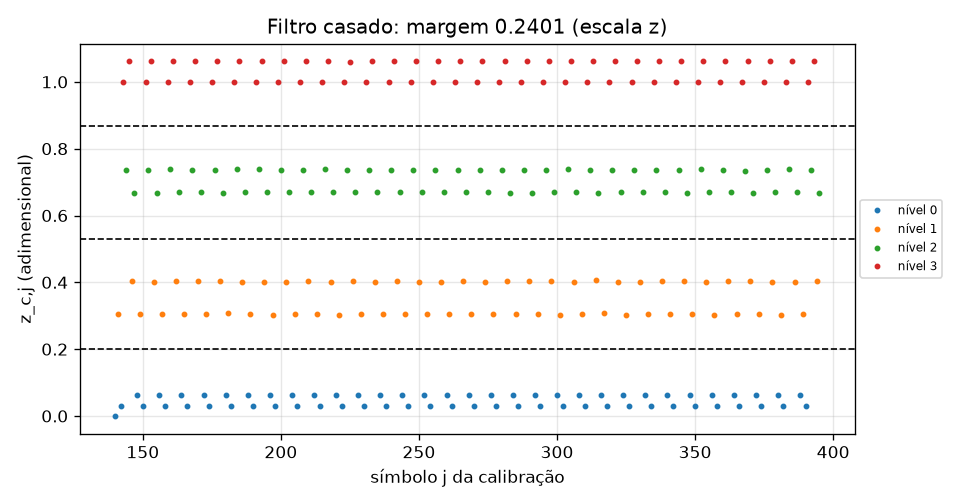
\includegraphics[width=\linewidth]{rx_RC16n8_PAM4_z.png}
        \caption{RC \SI{16,8}{nF}, PAM-4.}
    \end{subfigure}\hfill
    \begin{subfigure}{0.49\textwidth}\centering
        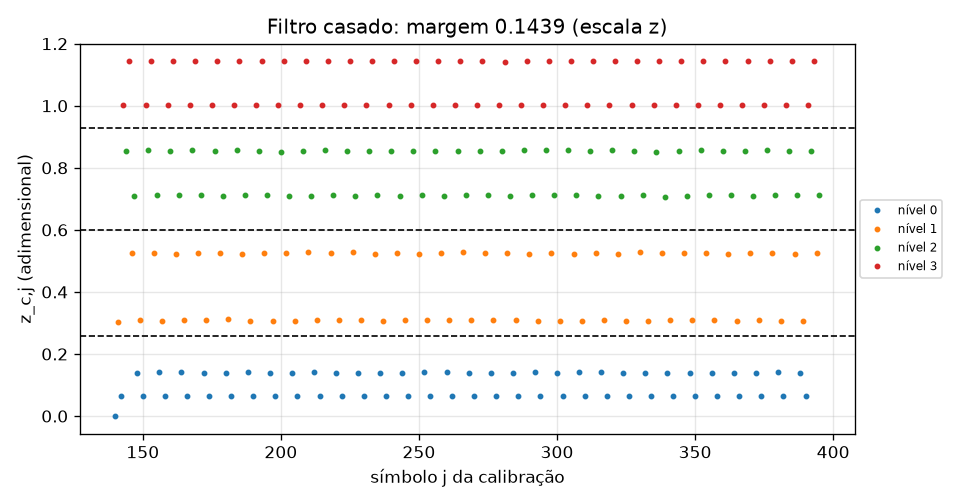
\includegraphics[width=\linewidth]{rx_RC33n_PAM4_z.png}
        \caption{RC \SI{33}{nF}, PAM-4.}
    \end{subfigure}
    \caption{Saída $z_{c,j}$ do filtro casado nos 256 símbolos de calibração, com os limiares. Cada
    nível se divide conforme o símbolo anterior (ISI); com \SI{33}{nF}, a separação entre níveis
    vizinhos cai.}
    \label{fig:z}
\end{figure}

\textbf{ISI no primeiro zero depois de A.} O RX registra a média das amostras do zero seguinte a A,
descontada a linha de base. Em $k=0$ ela vale \num{2585} códigos (\SI{2,08}{V}) com \SI{16,8}{nF} e
\num{3146} códigos com \SI{33}{nF}; em $k=7$ cai para \num{8.8} códigos (\SI{7}{mV}) e \num{137}
códigos (\SI{110}{mV}), respectivamente. No canal Dupont, o resíduo é inferior a 1 código. Esses
casos não foram retirados do payload.

\subsection{Contagem de erros, BER e SER}

A Tabela~\ref{tab:ber} corresponde à tabela da Seção 5.1 do enunciado. As contagens vêm dos
contadores do RX, sobre as mesmas amostras do payload para os dois detectores, depois da confirmação
dos 48 bits de início do quadro (0 erros nesses bits nos dois detectores em todos os quadros listados).

\begin{table}[H]
\centering
\caption{Registro dos resultados (Seção 5.1 do enunciado). Denominador da BER: \num{100000} bits.}
\label{tab:ber}
\small
\begin{tabular}{l c c c c c c c}
\toprule
Canal & PAM & Abertura & $\tau$ & \multicolumn{2}{c}{Amostra única} & \multicolumn{2}{c}{Filtro casado} \\
 & & (V) & (\si{\micro\second}) & $N_e$; BER & $N_s$; SER & $N_e$; BER & $N_s$; SER \\
\midrule
Dupont & 2 & 3,291 & 0,22 & 0; 0 & 0; 0 & 0; 0 & 0; 0 \\
Dupont & 4 & 0,965 & 0,21 & 0; 0 & 0; 0 & 0; 0 & 0; 0 \\
RC (\SI{16,8}{nF}) & 2 & 3,273 & 7,32 & 0; 0 & 0; 0 & 0; 0 & 0; 0 \\
RC (\SI{16,8}{nF}) & 4 & 0,979 & 7,30 & 0; 0 & 0; 0 & 0; 0 & 0; 0 \\
Cabo manga & 2 & 3,262 & 7,3$^\dagger$ & 0; 0 & 0; 0 & 0; 0 & 0; 0 \\
Cabo manga & 4 & 0,970 & -- & 0; 0 & 0; 0 & 0; 0 & 0; 0 \\
\midrule
RC (\SI{33}{nF}) & 2 & 2,989 & 13,20 & 0; 0 & 0; 0 & 0; 0 & 0; 0 \\
RC (\SI{33}{nF}) & 4 & 0,838 & 13,00 & 0; 0 & 0; 0 & 0; 0 & 0; 0 \\
\bottomrule
\multicolumn{8}{l}{\footnotesize $^\dagger$ indicativo (linha distribuída). SER: $N_{sym}=\num{100000}$ (PAM-2) e \num{50000} (PAM-4).}
\end{tabular}
\end{table}

Em todas as condições obrigatórias o resultado foi \textbf{0 erros em \num{100000} bits} para os dois
detectores, isto é, $\widehat{\text{BER}} = 0$ observada. Isso não demonstra BER física nula: com
zero erros em \num{100000} bits, o limite superior de 95\,\% é cerca de \num{3e-5} por quadro.
Considerando todos os quadros válidos registrados nos canais Dupont e RC \SI{16,8}{nF} entre 01 e
04/11/2026 (25 quadros, \num{2.5e6} bits por detector), também não houve nenhum erro, o que reduz
o limite superior para cerca de \num{1.2e-6}. Como as duas BER são nulas, as contagens não permitem
dizer qual detector é melhor nesses canais. A comparação é feita pelas margens (Tabela~\ref{tab:centros}):
uma margem maior não garante BER menor, mas indica maior folga contra ruído e interferência.

\textbf{Erro de bit $\times$ falha de quadro.} Um erro de bit é uma decisão errada num quadro em que
todas as amostras foram recebidas e o sincronismo foi confirmado. Uma falha de quadro (perda de CLK,
contagem de amostras errada, overrun ou palavra de sincronismo não reconhecida) invalida o quadro
inteiro, que não recebe BER. Ao longo do projeto, 29 quadros foram descartados por esse motivo,
todos detectados pelas verificações do firmware e repetidos (Seção~\ref{sec:dificuldades}). Nenhum
deles produziu uma BER falsa.

\subsection{Canal 3: cabo manga de \SI{200}{m} (exploratório)}
\label{sec:manga}

\textbf{Montagem e retorno de GND.} Os dados passaram pelo condutor A do cabo e o GND pelo condutor
B. O CLK seguiu por Dupont curto, o que exigiu um GND curto entre as placas. Além disso, as duas
placas estavam ligadas por USB ao mesmo PC (o RX através do Pico), e o osciloscópio, ligado ao PC e
à tomada, tinha os jacarés das pontas nos GND das duas placas (Figura~\ref{fig:manga_gnd}). O retorno
efetivo da corrente de dados se divide entre o condutor B e esses caminhos curtos em paralelo. Assim,
o ensaio representa principalmente um condutor longo de dados com referência próxima, e não um enlace
isolado de \SI{200}{m} para sinal e retorno. Também não se atribui ao cabo a integridade do CLK, que
percorreu apenas \SI{20}{cm}.

\begin{figure}[H]
    \centering
    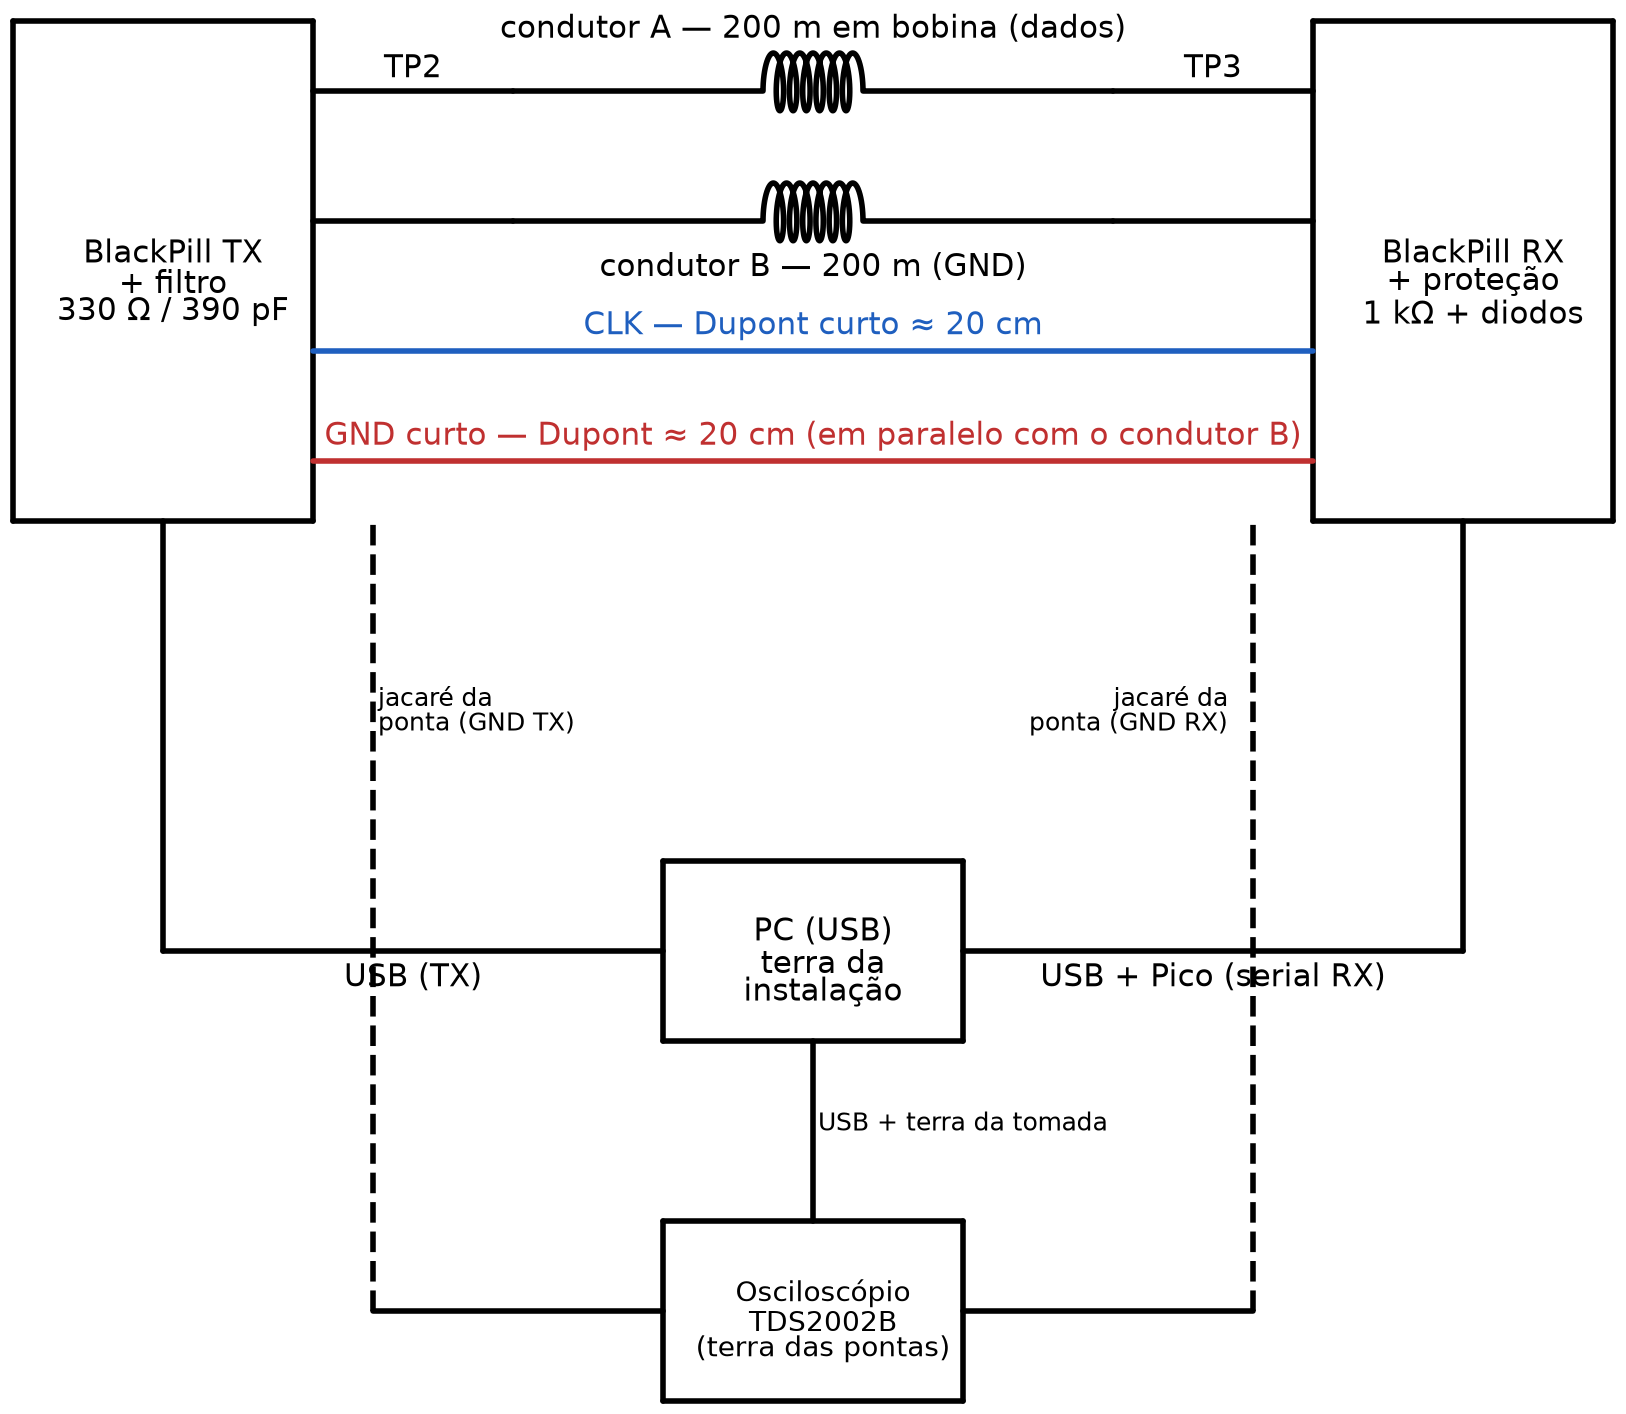
\includegraphics[width=0.75\textwidth]{manga_retorno_gnd.png}
    \caption{Caminhos reais de GND no ensaio do cabo manga.}
    \label{fig:manga_gnd}
\end{figure}

\textbf{Resultados.} Os dois quadros válidos finais (Tabela~\ref{tab:ber}) tiveram 0 erros nos dois
detectores, com aberturas de \SI{3,262}{V} (PAM-2) e \SI{0,970}{V} (PAM-4) em $k^\star = 7$. A
subida é rápida no início e tem cauda lenta (Figura~\ref{fig:degrau}d e $p_c[k]$ na
Tabela~\ref{tab:pc}), comportamento típico de uma linha RC distribuída: a resistência e a capacitância
estão espalhadas ao longo dos \SI{200}{m}, e por isso o ``$\tau$ de 63\,\%'' é apenas indicativo.
TP2 também é carregado pela capacitância do cabo (salto de cerca de 23\,\%). A razão de PSD
Manga/Dupont foi de 0,965 em \SI{5}{kHz} e 0,89 em \SI{10}{kHz}: o cabo atenua menos que o RC de
\SI{16,8}{nF} em \SI{10}{kHz}. O olho é visivelmente mais ruidoso que nos outros canais
(Figura~\ref{fig:olhos}d), o que é coerente com o condutor longo em bobina captando interferência.

\textbf{Falhas documentadas.} (i) Quatro quadros foram perdidos por \texttt{perda\_CLK} durante o
ensaio do cabo, sempre detectados pelo RX. (ii) O primeiro quadro PAM-4 válido
(\texttt{Manga\_PAM4\_20261103\_165336}, Figura~\ref{fig:manga_anom}) teve abertura de apenas
\SI{0,589}{V}, linha de base $b_c$ de \SI{110}{mV} e \textbf{14 erros no filtro casado}
($\widehat{\text{BER}} = \num{1.4e-4}$, $\widehat{\text{SER}} = \num{2.8e-4}$), contra 0 erros na
amostra única no mesmo quadro. Nesse quadro, o degrau chegou a apenas 84\,\% do valor final em
$k^\star$, e a margem relativa do filtro caiu para 0,28, contra 0,64 da amostra única. O
comportamento não se repetiu nos quadros seguintes. A hipótese mais provável é um mau contato
momentâneo na conexão do cabo ou do retorno de GND. Esse quadro mostra, com dados, que o filtro casado
treinado num pulso isolado é mais sensível a distorção e ISI do que a amostra única no fim do símbolo.

\begin{figure}[H]
    \centering
    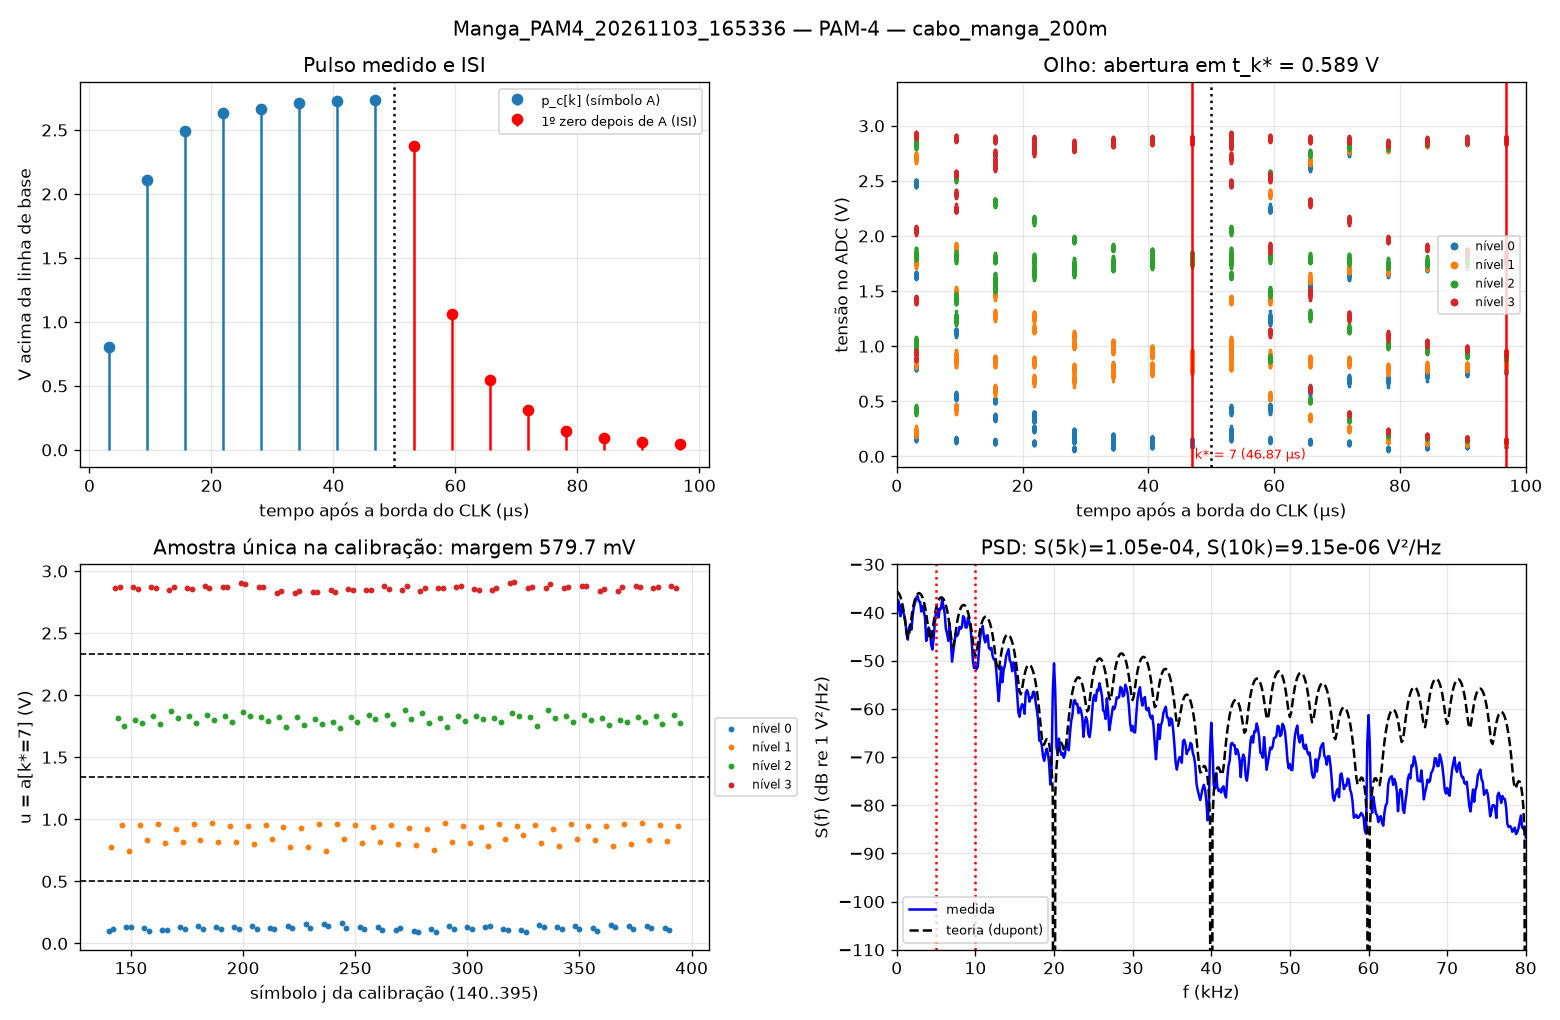
\includegraphics[width=0.92\textwidth]{rx_Manga_PAM4_anomalia.png}
    \caption{Quadro anômalo no cabo manga (PAM-4): olho fechado nas primeiras posições, margem menor
    e 14 erros no filtro casado (0 na amostra única).}
    \label{fig:manga_anom}
\end{figure}

\subsection{Verificação ao vivo: capacitor de \SI{33}{nF}}

Trocar apenas o capacitor do canal 2 de \SI{16,8}{nF} para \SI{33}{nF} produziu: $\tau$ de 7,30 para
\SI{13,0}{\micro\second} (fator 1,78, próximo de $33/16{,}8 = 1{,}96$ descontado o segundo polo fixo
do TX); tempo de subida de 16,2 para \SI{27,4}{\micro\second}; abertura PAM-4 em $k^\star$ de 0,979
para \SI{0,838}{V} (PAM-2: 3,273 para \SI{2,989}{V}); margem relativa do filtro de 0,73 para 0,44; e
razão de PSD em \SI{10}{kHz} de 0,81 para 0,55. Todas as mudanças vêm do mesmo fato: $f_c$ caiu de
cerca de \SI{22}{kHz} para cerca de \SI{12}{kHz}, então as componentes de frequência mais alta são
mais atenuadas, a subida fica mais lenta e uma fração maior de cada símbolo ainda carrega o símbolo
anterior. Mesmo assim, ambos os detectores tiveram 0 erros em \num{100000} bits. O capacitor de
\SI{33}{nF} é uma alteração didática, não o modelo nominal de \SI{300}{m}.

\begin{figure}[H]
    \centering
    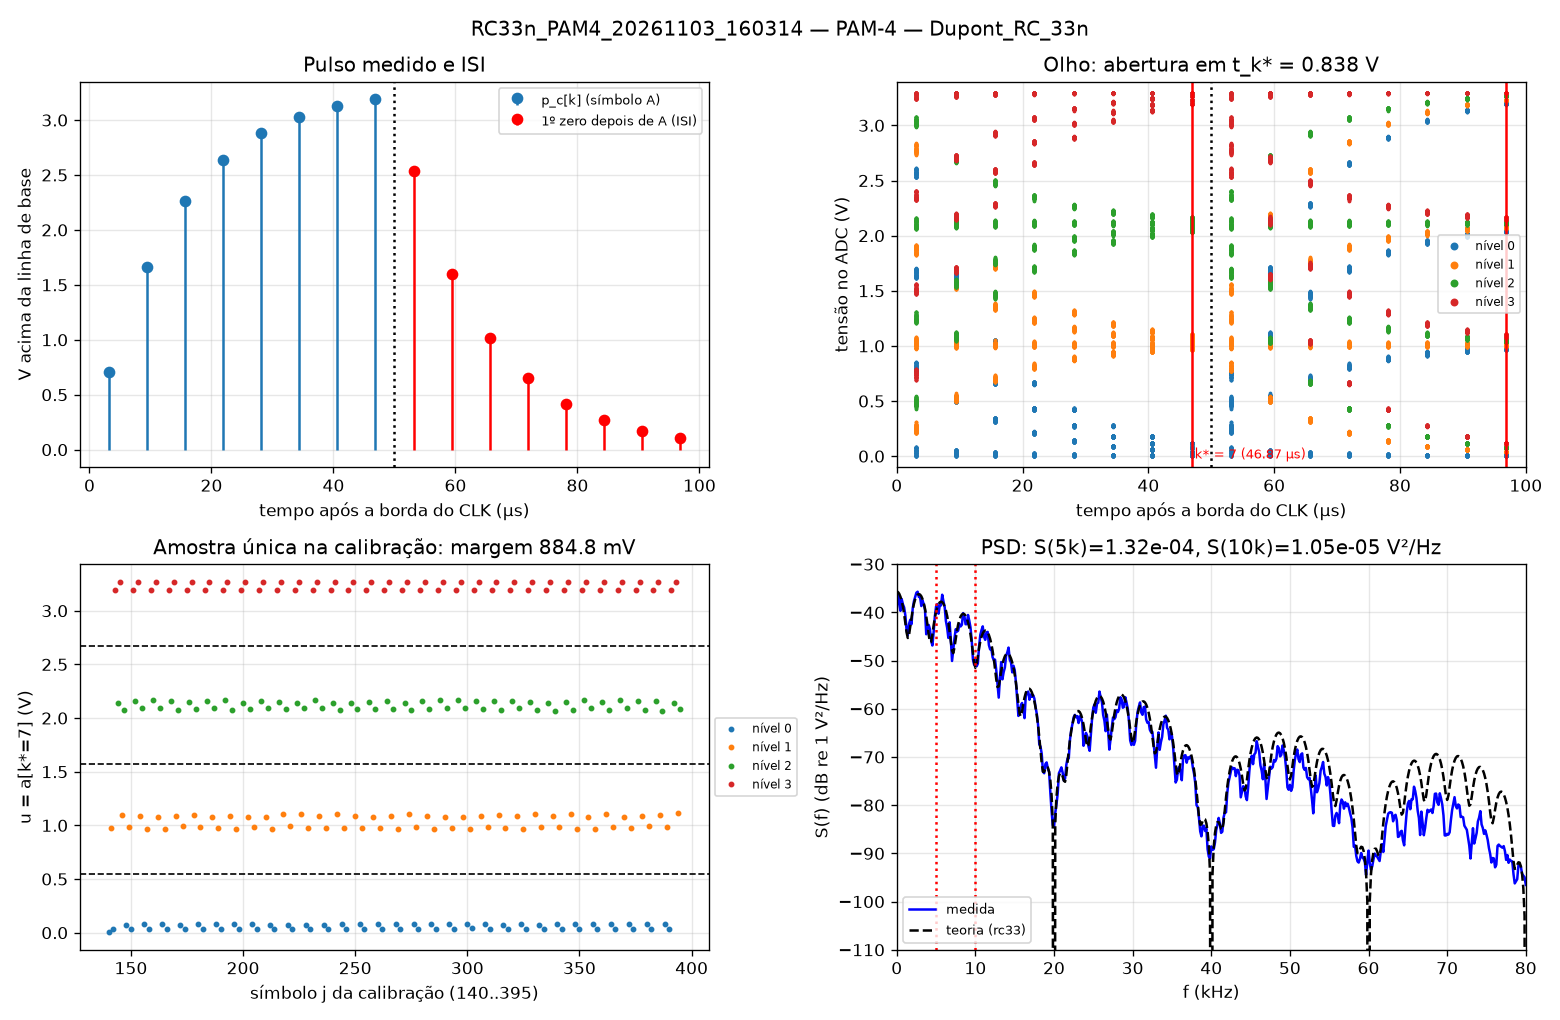
\includegraphics[width=0.92\textwidth]{rx_RC33n_PAM4.png}
    \caption{Análise do quadro RC \SI{33}{nF}, PAM-4: ISI maior no zero depois de A, olho fechado
    até $k=2$ e PSD mais atenuada.}
    \label{fig:rx_33}
\end{figure}

\subsection{Mesma taxa de bits: PAM-2 $\times$ PAM-4}

Para $R_b = \SI{20}{kbit/s}$, PAM-2 precisa de $R_s = \SI{20}{ksym/s}$ ($T_s = \SI{50}{\micro\second}$)
e PAM-4 de apenas $R_s = \SI{10}{ksym/s}$ ($T_s = \SI{100}{\micro\second}$). Com o PAM-4 mais lento,
o primeiro nulo espectral cai para \SI{10}{kHz} (metade da banda) e o resíduo de ISI com
\SI{33}{nF} passaria de $e^{-50/13} \approx 2$\,\% para $e^{-100/13} \approx 0{,}05$\,\%. Em
contrapartida, para a mesma excursão de \SI{3,3}{V}, os níveis PAM-4 ficam a 1/3 da distância dos
níveis PAM-2 (cerca de \SI{-9,5}{dB} de margem contra ruído). Esse ensaio a \SI{10}{ksym/s} é
opcional e não foi realizado. Na mesma taxa de símbolos (\SI{20}{ksym/s}), os dados mostram que o
PAM-4 dobra a taxa de bits ao custo de uma margem cerca de 3,4 vezes menor (\SI{0,98}{V} contra
\SI{3,28}{V} no RC \SI{16,8}{nF}).

\subsection{Dificuldades e diagnóstico}
\label{sec:dificuldades}

\begin{itemize}
    \item \textbf{CLK instável.} Quadros descartados por \texttt{perda\_CLK} (CLK interrompido por mau
    contato no fio PB4$\to$PA0 ou por RESET repetido) e por bordas a mais (por exemplo, \num{50442} e
    \num{50428} bordas para \num{50420} esperadas). Num caso, bordas falsas apareceram sem ninguém
    mexer na montagem, com o fio de CLK ao lado do fio de dados e sem a ponta do osciloscópio em PB4.
    A causa provável é diafonia dados$\to$CLK na entrada PA0 de alta impedância. Solução: fio de CLK
    curto e firme, afastado do fio de dados e com um fio de GND ao lado. Depois da correção, o quadro
    de teste na condição que falhava (\texttt{Dupont\_PAM4\_20261103\_163642}, sem ponta no CLK) recebeu
    \num{50420} de \num{50420} bordas, com sincronismo confirmado e 0 erros.
    \item \textbf{Mau contato na proteção do ADC.} Dois quadros RC \SI{33}{nF} PAM-2 tiveram níveis
    ``puxados para a média'' no ADC. A causa foi contato ruim em série com o ADC (\SI{1}{k\ohm}/TP4/PA1),
    corrigido antes do quadro válido.
    \item \textbf{Modo USB do osciloscópio.} O TDS2002B às vezes se apresentava ao PC como dispositivo
    HID em vez de USBTMC. Isso foi corrigido em \textit{Utility $\to$ Options $\to$ Rear USB Port
    $\to$ Computer}.
\end{itemize}

\subsection{Itens opcionais não realizados}

O desafio a \SI{100}{ksym/s}, a perturbação com GPIO e PRBS-7 e a medição a \SI{10}{ksym/s} não
foram realizados.

% ==================== SEÇÃO 5: CONCLUSÃO ====================
\section{Conclusão}

O enlace TX/RX foi implementado conforme o enunciado e verificado com medidas: CLK de
\SI{20,0008}{kHz} com 50\,\% de ciclo de trabalho, ordem Gray correta, oito amostras por símbolo
(\num{160000} amostras/s) sem perdas em todos os quadros válidos e quadros completos de
\num{100444} (PAM-2) e \num{50420} (PAM-4) símbolos com início de quadro confirmado.

\textbf{Canal 1 (Dupont).} O canal é transparente na escala do símbolo ($\tau < \SI{0,3}{\micro\second}
\ll T_s$): o olho fica aberto em todas as posições $k$, não há ISI mensurável, os dois detectores têm
a mesma margem relativa e o resultado foi 0 erros em \num{100000} bits em PAM-2 e PAM-4. A abertura
PAM-4 (\SI{0,965}{V}) é limitada pelo menor degrau de nível do TX (0--1) e a de PAM-2, pela saturação
do ADC em $V_{ref}$.

\textbf{Canal 2 (RC \SI{16,8}{nF}).} $\tau$ medido de \SI{7,30}{\micro\second}, contra
\SI{6,48}{\micro\second} pelo modelo simplificado e \SI{7,1}{\micro\second} considerando o filtro do
TX. A razão de PSD (0,945 em \SI{5}{kHz} e 0,81 em \SI{10}{kHz}) concorda com $|H(f)|^2$ para o
$\tau$ medido e independe da modulação. O olho só abre plenamente no fim do símbolo ($k^\star=7$), e
a abertura no instante escolhido praticamente não muda em relação ao Dupont (\SI{0,979}{V} em PAM-4).
Houve 0 erros em \num{100000} bits nos dois detectores. A margem relativa do filtro casado
(0,73 em PAM-4) já é menor que a da amostra única (0,90). Em ambos os canais principais, a amostra
única em $k^\star$ foi o detector com maior folga, e o PAM-2 teve margem cerca de 3,4 vezes maior que
o PAM-4, ao custo de metade da taxa de bits.

\textbf{Canal 3 (cabo manga, exploratório).} Houve comunicação com 0 erros nos quadros válidos finais,
mas com olho mais ruidoso, perdas de CLK e um quadro anômalo com 14 erros só no filtro casado. Esses
resultados representam um condutor longo de dados com referência de GND próxima.

\textbf{Troca para \SI{33}{nF}.} $\tau$ de \SI{13,0}{\micro\second}, tempo de subida de
\SI{27,4}{\micro\second}, abertura PAM-4 de \SI{0,838}{V}, razão de PSD de 0,55 em \SI{10}{kHz} e
margem relativa do filtro de 0,44 mostram, com números próprios, como a redução da banda do canal se
traduz em ISI e no fechamento do olho. Mesmo assim, não houve erros em \num{100000} bits.

Em resumo, com o baixo ruído desta bancada, o fator limitante foi a ISI e não o ruído. Por isso, o
detector de amostra única no fim do símbolo superou o filtro casado em margem. A ausência de erros nos
quadros válidos permite afirmar apenas que a BER é inferior a cerca de \num{3e-5} por condição (95\,\%
de confiança), e não que ela seja nula.

% ==================== SEÇÃO 6: USO DE IA ====================
\section{Uso de inteligência artificial e origem das informações}

Conforme a Seção 3 do enunciado, informa-se o uso de IA. Foi usado o assistente Claude (Anthropic),
por meio da ferramenta Claude Code, nas seguintes partes:
\begin{itemize}
    \item planejamento das etapas, roteiro de bancada e material de estudo para a defesa;
    \item redação de versões iniciais dos módulos de firmware (\texttt{pam\_frame}, \texttt{pam\_tx},
    \texttt{pam\_rx}, \texttt{pam\_rx\_core}, \texttt{pam\_rx\_report}), integrados pelo autor aos
    projetos do STM32CubeIDE;
    \item scripts de análise em Python e MATLAB (PSD, $\tau$, olho, tabelas), automação do osciloscópio
    pela USB e modelos Simulink de referência;
    \item organização dos dados e redação deste relatório a partir dos registros da bancada.
\end{itemize}
O autor foi responsável pela configuração dos projetos \texttt{.ioc}, pela montagem dos circuitos,
pela gravação e depuração das placas, pela execução de todos os ensaios, pela verificação dos
resultados e pelas conclusões, e responde pela correção do circuito, do código e dos resultados.

\textbf{Parâmetros do enunciado:} $T_s$, PWM (PSC, ARR, CCR), TIM2 (ARR\,=\,624, CCR2\,=\,312),
configuração do ADC/DMA, PRBS-15, estrutura do quadro e palavra de sincronismo, mapeamento Gray,
valores nominais de R e C dos canais, procedimento de escolha de $k^\star$, equação do filtro casado e
método da PSD.

\textbf{Dependem de medições próprias:} $V_{ref}$, níveis em TP2, frequência do CLK, ripple,
atraso CLK--dados, todos os valores de $\tau$ e tempo de subida, aberturas, $k^\star$, $p_c[k]$,
centros, limiares, margens, PSDs e razões, contagens de erros, falhas registradas e todas as
conclusões das Seções 4 e 5.

% ==================== APÊNDICE ====================
\appendix
\section{Checklist dos entregáveis e localização dos arquivos}

\begin{table}[H]
\centering
\small
\begin{tabularx}{\textwidth}{c X l}
\toprule
Feito & Material & Onde \\
\midrule
$\checkmark$ & Código-fonte e \texttt{.ioc} do TX e do RX & \nolinkurl{firmware/fir_tx/TX}, \nolinkurl{firmware/fir_tx/RX} \\
$\checkmark$ & TX PAM-2/PAM-4: níveis em TP2, CLK de \SI{50}{\micro\second}, ordem Gray & Fig.~\ref{fig:tx}, \ref{fig:tx_pam2}; \nolinkurl{entrega/capturas/TX_*} \\
$\checkmark$ & RX: oito amostras por símbolo, \num{160000} amostras/s, perdas & Tab.~\ref{tab:logs}; logs \\
$\checkmark$ & Olhos em TP3 com $k^\star$, instante e abertura (4 condições) & Fig.~\ref{fig:olhos}, \ref{fig:rx}, \ref{fig:rx_rc}; Tab.~\ref{tab:olho} \\
$\checkmark$ & Transições em TP2 e TP3; $t_{10-90}$ e $\tau$ & Fig.~\ref{fig:degrau}; Tab.~\ref{tab:tau} \\
$\checkmark$ & PSD PAM-2/PAM-4, Dupont e RC, com \num{8192} amostras brutas & Fig.~\ref{fig:psd}; Tab.~\ref{tab:psd}; bloco \texttt{\#BEGIN\_PSD} dos logs \\
$\checkmark$ & Método da PSD & Seção~\ref{sec:metpsd} \\
$\checkmark$ & $p_c[k]$, $k^\star$, centros, limiares, margens, erros, BER e SER (4 condições) & Tab.~\ref{tab:pc}, \ref{tab:centros}, \ref{tab:ber} \\
$\checkmark$ & Cabo manga: forma de onda, olho, sincronismo, retorno de GND, BER & Seção~\ref{sec:manga} \\
$\checkmark$ & Comparação, conclusão por canal, registros brutos e uso de IA & Seções 4--6; \nolinkurl{entrega/} \\
\bottomrule
\end{tabularx}
\end{table}

Registros brutos: \nolinkurl{entrega/logs/} (relatórios completos do RX, incluindo as 256 janelas
de calibração e as \num{8192} amostras de PSD; quadros inválidos em \nolinkurl{entrega/logs/invalidos/}),
\nolinkurl{entrega/capturas/} (telas e CSV dos dois canais do osciloscópio),
\nolinkurl{entrega/CADERNO_BANCADA.md} (caderno de bancada gerado durante os ensaios) e
\nolinkurl{entrega/tabela_resultados_20261103.csv}. A análise pode ser refeita com
\texttt{python/pam\_app.py analisar <log> --vref 3.297}.

% ==================== REFERÊNCIAS ====================
\begin{thebibliography}{9}

\bibitem{enunciado}
KRAUSS, Roberto. \textit{Telecomunicações -- Projeto: transmissão PAM em banda base. Enunciado da
avaliação prática}. Campo Mourão: UTFPR, 2026.

\bibitem{haykin}
HAYKIN, Simon; MOHER, Michael. \textit{Sistemas de Comunicação}. 5. ed. Porto Alegre, RS: Bookman, 2011.

\bibitem{lathi}
LATHI, B. P.; DING, Z. \textit{Sistemas de Comunicações Analógicos e Digitais Modernos}. 4. ed. Rio de
Janeiro: LTC, 2019.

\bibitem{rm0383}
STMICROELECTRONICS. \textit{RM0383: STM32F411xC/E advanced Arm-based 32-bit MCUs -- Reference manual}.

\bibitem{tds}
TEKTRONIX. \textit{TDS1000B and TDS2000B Series Digital Storage Oscilloscopes -- User Manual}.

\bibitem{belden}
BELDEN. \textit{1583E -- Category 5e cable: technical data sheet}.

\end{thebibliography}

\end{document}
